%%
%%  Hochschule für Technik und Wirtschaft Berlin --  Abschlussarbeit
%%
%%  Hauptdokument
%%
%%%%%%%%%%%%%%%%%%%%%%%%%%%%%%%%%%%%%%%%%%%%%%%%%%%

%% Einstellungen und Anpassungen
% Wichtige Pakete und Grundeinstellungen, verwendet Dokumentenklasse "scrbook" 
\documentclass[
		chapterprefix=false, 
		12pt, 
		a4paper, 
		twoside, 
		parskip=half, 
		listof=totoc, 
		bibliography=totoc, 
		numbers=noendperiod, 
		captions=tableheading
]{scrbook}

%Anpassung der Seitenränder 
%% Geometrisches ...
\usepackage{geometry}
\makeatletter
\setlength\paperheight     {297mm}
\setlength\paperwidth  	   {210mm}
\setlength\headheight      {2ex}
\setlength\headsep         {4ex} %2
\setlength\footskip        {35pt} %25
\setlength\textwidth       {150mm}
\setlength\textheight      {240mm} %245
\setlength{\@tempdima}     {\paperwidth}
\addtolength{\@tempdima}   {-2in}
\addtolength{\@tempdima}   {-\textwidth}
\setlength\oddsidemargin   {0.5\@tempdima}
\setlength\evensidemargin  {\oddsidemargin}
\setlength{\@tempdima}     {\paperheight}
\addtolength{\@tempdima}   {-3in}
\addtolength{\@tempdima}   {-\textheight}
\setlength\topmargin       {.5\@tempdima}
\setlength\footnotesep     {12\p@}
\setlength{\skip\footins}  {10\p@ \@plus 2\p@ \@minus 4\p@}
\setlength{\marginparsep}  {1pt}
\setlength{\marginparwidth}{20mm}
\makeatother 


%% Unterstützung von Umlauten und anderen Sonderzeichen (UTF-8)
\usepackage{lmodern}
\usepackage{eurosym}
\usepackage[utf8]{inputenc}
\usepackage[T1]{fontenc}
\DeclareUnicodeCharacter{20AC}{\euro} %Euro-Symbol in UTF-8

%% Allgemeine Anpassungen 
\usepackage{scrhack} %Tweaks für scrbook
\usepackage[automark,headsepline]{scrlayer-scrpage} %Anpassung von Kopf- und Fußzeile
\usepackage{paralist}  %Kompakte Listen
\usepackage[onehalfspacing]{setspace} %Zeilenabstand 1,5
\usepackage[stretch=10]{microtype} %Verbesserte Darstellung der Buchstaben zueinander
\usepackage{float} %Unterstützung fester Positionierung  (H)
\usepackage{csquotes} %wird von babel benötigt

\usepackage{changepage} % Margin adjustment and detection of odd/even pages
\usepackage{blindtext}

%Glossar, Stichworverzeichnis (Akronyme als eigene Liste)
%\usepackage[toc, acronym]{glossaries} 

%% Mathematik:
\RequirePackage{amssymb, amsmath}
\RequirePackage{ifthen}
\RequirePackage{pifont} % Zapf Dingbats : https://ctan.ebinger.cc/tex-archive/macros/latex/required/psnfss/psnfss2e.pdf

%% Erweiterte Tabellen:
\usepackage{array, tabularx}
\usepackage{multirow}
\usepackage{longtable} %Umbrüche in Tabellen
\usepackage{booktabs}

%% Grafiken:
% Definition eigener Farben 
\usepackage[table,xcdraw]{xcolor}
\usepackage{tikz} % Vektorgrafiken, lädt graphicx automatisch
\usepackage{bmpsize} 

%Verknüpfungen im Dokument, Links werden durch "hidelink" nicht explizit hervorgehoben
%\PassOptionsToPackage{hyphens}{url}
\usepackage[hidelinks,german]{hyperref}
%\hypersetup{breaklinks=true}
\usepackage{breakurl}
%\expandafter\def\expandafter\UrlBreaks\expandafter{\UrlBreaks% save the current one
%  \do\a\do\b\do\c\do\d\do\e\do\f\do\g\do\h\do\i\do\j%
%  \do\k\do\l\do\m\do\n\do\o\do\p\do\q\do\r\do\s\do\t%
%  \do\u\do\v\do\w\do\x\do\y\do\z\do\A\do\B\do\C\do\D%
%  \do\E\do\F\do\G\do\H\do\I\do\J\do\K\do\L\do\M\do\N%
%  \do\O\do\P\do\Q\do\R\do\S\do\T\do\U\do\V\do\W\do\X%
%  \do\Y\do\Z\do\*\do\-\do\~\do\'\do\"\do\-}%
\usepackage{import}
  		% Import der Pakete und Stil des Dokuments
%%% Einstellungen zur Sprache und Silbentrennung im Dokument
%
% This is a document holding multiple languages.
% Switch between ENGLISH and GERMAN by commenting one of the following lines:
%\usepackage[ngerman,english]{babel} % makes ENGLISH content
\usepackage[english,ngerman]{babel} % makes GERMAN content
% this is the macro to define phrases in two languages:
\newcommand{\babel}[2]{\ifnum\pdfstrcmp{\languagename}{english}=0 {#2}\else{#1}\fi}
\newcommand{\DE}[1]{\ifnum\pdfstrcmp{\languagename}{ngerman}=0 {#1}\fi}
\newcommand{\EN}[1]{\ifnum\pdfstrcmp{\languagename}{english}=0 {#1}\fi}
% example:   \babel{Deutscher Text}{english text}
% example:   \DE{deutscher Text}
% example:   \EN{english text}
%%%%%%%%%%%%%%%


%%% Erstellung von Literaturverzeichnissen mit Biblatex (Biber/Bibtex)
% wählen Sie hier die für Ihr Latex-System nötige Literaturverarbeitung:
% \usepackage[style=alphabetic, backend=biber,   natbib=true]{biblatex}  % Verarbeitung mit biber
\usepackage[style=alphabetic, backend=bibtex, natbib=true]{biblatex}  % Verarbeitung mit bibtex
%
% Bibtex-Datei mit den Quellenangaben zur Arbeit
\addbibresource{references/references.bib}


%%% Abkürzungsverzeichnis
\usepackage[intoc]{nomencl}
\let\acro\nomenclature
\renewcommand{\nomname}{\babel{Abkürzungsverzeichnis}{Abbreviations}}
\setlength{\nomlabelwidth}{.25\hsize}
\renewcommand{\nomlabel}[1]{#1 \dotfill}
\setlength{\nomitemsep}{-\parsep}
\makenomenclature

%%% Überschriften auch in Times-Roman setzen
\addtokomafont{disposition}{\rmfamily}

%%% Kapitelnummer und Titel auf einer Zeile (erfordert die chapterprefix=false Option in class)
\renewcommand*{\chapterformat}{%
  \mbox{\chapapp~\thechapter:\enskip}%
}

%%% Farbdefinitionen
%  https://corporatedesign.htw-berlin.de/schrift-farbe/markenfarben/
\definecolor{HKS66}{RGB}{118,185,0}          %% HKS51, HTW-Grün
\definecolor{HKS47}{RGB}{0,130,209}      %% HKS47, HTW-Blau
\newcommand{\headcolor}{HKS66}
\newcommand{\alertcolor}{HKS47}
% Zusätzliche Farben
\definecolor{darkgreen}{RGB}{0,100,0}


%%% Stichwortverzeichnis 
\usepackage{imakeidx}
\makeatletter
\makeindex[columns=2, title=\babel{Stichwortverzeichnis}{Index}, options= -s settings/indexstyle.ist, intoc]
\makeatother
\indexsetup{level=\chapter*,toclevel=chapter}
% Pluszeichen in der Referenz beim Zitieren entfernen: [Kra+13] wird zu [Kra13]
\renewcommand*{\labelalphaothers}{}


%%% Darstellung von Quellcode incl. Syntax-Highlighting
\usepackage{listings}
\renewcommand{\lstlistlistingname}{\babel{Quelltextverzeichnis}{Listings}}
%Anpassungen zur Quellcodedarstellung
% muss bei Bedarf überschrieben werden (z.B. wenn unterschiedliche Sprachen zum Einsatz kommen)
\renewcommand{\lstlistingname}{Codeauszug}
\lstset{
	language=Java,
	numbers=left,
	columns=fullflexible,
	aboveskip=5pt,
	belowskip=10pt,
	basicstyle=\small\ttfamily,
	backgroundcolor=\color{black!5},
	commentstyle=\color{darkgreen},
	keywordstyle=\color{blue},
	stringstyle=\color{gray},
	showspaces=false,
	showstringspaces=false,
	showtabs=false,
	xleftmargin=16pt,
	xrightmargin=0pt,
	framesep=5pt,
	framerule=3pt,
	frame=leftline,
	rulecolor=\color{green},
	tabsize=2,
	breaklines=true,
	breakatwhitespace=true,
	prebreak={\mbox{$\hookleftarrow$}}
}

 	% Weitere Pakete und Anpassungen (Sprache, Quellenverwaltung, etc.)

% Variablendefinition und deren Voreinstellung festlegen
%

%% Variablen
\newboolean{@entwurfset}        \setboolean{@entwurfset}{true}
\newboolean{@abgabeset}         \setboolean{@abgabeset}{true}
\newboolean{@versionset}        \setboolean{@versionset}{true}
\newboolean{@versionsdatum}      \setboolean{@versionsdatum}{true}

%
\newcommand{\version}[1]{\setboolean{@versionset}{true} 
 \renewcommand{\theversion}{#1}} 
\newcommand{\datum}[1]{\renewcommand{\thedatum}{#1}}
\newcommand{\autor}[1]{\renewcommand{\theautor}{#1}}
\newcommand{\matrikelnr}[1]{\renewcommand{\thematrikelnr}{#1}}
\newcommand{\titel}[1]{\renewcommand{\thetitel}{#1}}
\newcommand{\untertitel}[1]{\renewcommand{\theuntertitel}{#1}}
\newcommand{\fachbereich}[1]{\renewcommand{\thefachbereich}{#1}}
\newcommand{\studiengang}[1]{\renewcommand{\thestudiengang}{#1}}
\newcommand{\thesistyp}[1]{\renewcommand{\thethesistyp}{#1}}
\newcommand{\abschluss}[1]{\renewcommand{\theabschluss}{#1}}
\newcommand{\firstExaminer}[1]{\renewcommand{\thefirstExaminer}{#1}}
\newcommand{\secondExaminer}[1]{\renewcommand{\thesecondExaminer}{#1}}
\newcommand{\betreuerFeld}[1]{\renewcommand{\thebetreuerFeld}{#1}}

%
\newcommand{\theversion}{0.0}      
\newcommand{\thedatum}{\today}
\newcommand{\theautor}{Autor angeben!}
\newcommand{\thematrikelnr}{123 456}
\newcommand{\thetitel}{Titel angeben!}
\newcommand{\theuntertitel}{}
\newcommand{\thefachbereich}{Fachbereich angeben}
\newcommand{\thestudiengang}{Studiengang angeben}
\newcommand{\thethesistyp}{Bachelorarbeit}
\newcommand{\theabschluss}{Bachelor of Engineering (B.Eng.)}
\newcommand{\thefirstExaminer}{Betreuer 1}
\newcommand{\thesecondExaminer}{Betreuer 2}
\newcommand{\thebetreuerFeld}{}

\betreuerFeld{
  \begin{tabular}{llr}
    Erstgutachten und Betreuung: & \thefirstExaminer \\
    Zweitgutachten: & \thesecondExaminer \\
  \end{tabular}
}

%%%%%%%%%%%%%%%%%%%%%%%%%%%%%%%%
\renewcommand{\maketitle}{\htwTitelSeite}

%% Optionen

\DeclareOption{entwurf}
    {
      \setboolean{@entwurfset}{true}
      \setboolean{@abgabeset}{false}
    }

\DeclareOption{abgabe}
    {
      \setboolean{@entwurfset}{false}
      \setboolean{@abgabeset}{true}
    }



%% Setzen des defaults und verarbeiten
\ExecuteOptions{abgabe}     %TODO für Abgabe auf abgabe setzen
\ProcessOptions 

%%%%%%%%%%%%%%%%%%%%%%%%%%%%%%%%
%\newcommand{\hslogo}{pictures/Logo_HTW_Berlin.pdf}
%\newcommand{\hslogoscaled}[1]{{\mbox{\includegraphics[width=#1]\hslogo}}}

\newcommand{\hsfont}{}%    {\fontfamily{phv}\fontseries{m}\fontshape{n}\selectfont}
\newcommand{\hsheadfont}{}%{\fontfamily{phv}\fontseries{b}\fontshape{n}\selectfont}

\newcommand{\htwTitelSeite}
    {
      \thispagestyle{empty}
      \parindent=0pt
      \begin{minipage}[b]{0.65\textwidth}
       
        \ifthenelse{\boolean{@entwurfset}}
            {
              \begin{hsfont}
                \begin{tiny}
                  \raggedright
                  % Versionsnummer, wenn gesetzt
                  \ifthenelse{\boolean{@versionset}}
                       {Version \theversion\\}
                       {}
                       % Datum der letzten Änderung, falls gewünscht
	               \ifthenelse{\boolean{@versionsdatum}}
                       {letzte Änderung: \today \\}
		       {}
                \end{tiny}
              \end{hsfont}
            }
            {              
              % leer
              ~\hfill~
            }
      \end{minipage}
      
      \begin{minipage}[b]{0.35\textwidth}
      \vskip -2em
      \hfill  %\hslogoscaled{\textwidth}
%      \Ifpdfoutput{
%                  \message{PDF Output}
                  \mbox{
\includegraphics[width=\textwidth]{pictures/Logo_HTW_Berlin}}
%                  }{
%                 \mbox{
\includegraphics[width=\textwidth]{pictures/Logo_HTW_Berlin.eps}}
%                  \message{Kein PDF Output}
%                  }
      \end{minipage}

      \textcolor{HKS66}{\rule{\linewidth}{.4mm}}
      \vspace*{\stretch{1}}
      \begin{center}
        \begin{hsheadfont}
          \textcolor{\headcolor}{\LARGE \textbf{\thetitel}}
        \end{hsheadfont}
      \end{center}
      \vspace*{\stretch{0.5}}
      %
      \begin{hsheadfont}
        \begin{center}
          \textbf{\Large{\thethesistyp}}
        \end{center}
      \end{hsheadfont}
      \vspace*{\stretch{0.5}}
      %
      \begin{center}
        \begin{hsfont}
          von\\[2ex]
          {\textbf{\large\theautor}}\\[2ex]
          Matrikelnummer: \thematrikelnr\\[2ex]
          Fachbereich \thefachbereich\\
          der Hochschule für Technik und Wirtschaft Berlin\\[2ex]
          zur Erlangung des akademischen Grades\\
          \textbf{\theabschluss}\\
          im Studiengang\\
          \textbf{\thestudiengang}
        \end{hsfont}
      \end{center}
     
      \vspace*{\stretch{1}}
       \begin{center}
         Tag der Abgabe: \thedatum 
       \end{center}
         
      \vspace*{\stretch{1}}
      
      \thebetreuerFeld
      
      %
      \vspace*{\stretch{2}}

      \textcolor{HKS66}{\rule{\linewidth}{0.4mm}}\\[1.5ex]
       \begin{hsheadfont}
         % leer
         ~\hfill~
       \end{hsheadfont}
    }
		% Layout der Titelseite

%%%%%%%%%%%%%%%%%%%%%%%%%%%%%%%%%%%%%%%%%%%%%
%%%%%%%%%%%%%%%%%%%%%%%%%%%%%%%%%%%%%%%%%%%%%
%% In diesem Bereich müssen Sie Anpassungen für das Deckblatt der Arbeit vornehmen!
%
%% Titel und Author 
\titel{Luftfeuchtigkeits-Sensornetzwerk zur zeitnahen Detektion von Wasserschäden auf Basis von LoRa(WAN)}
\autor{Sidney Göhler und Ilja Buschujew}
% \matrikelnr{s0559016}
%% Version und Abgabedatum
\version{0.2$\alpha$} 	%ToDo: wird derzeit noch nicht genutzt
\datum{25.02.2022}   	% Abgabedatum der Arbeit
%% Typ der Arbeit
\thesistyp{Projektabschlussbericht}
%\thesistyp{Bachelorarbeit}
\abschluss{Projekt Netzbasierte Systeme}
%\abschluss{Bachelor of Engineering (B. Eng.)}
%% Betreuer
\firstExaminer{Prof.~Dr. Thomas Scheffler}
\secondExaminer{Hanna Full}
%% Fachbereich
\fachbereich{1 -- Energie und Information --}
\studiengang{Informations- und Kommunikationstechnik (M. Eng.)}
%%%%%%%%%%%%%%%%%%%%%%%%%%%%%%%%%%%%%%%%%%%%%
%%%%%%%%%%%%%%%%%%%%%%%%%%%%%%%%%%%%%%%%%%%%%
%%%%%%%%%%%%%%%%%%%%%%%%%%%%%%%%%%%%%%%%%%%%%s

%% Pfad zu den Bildern
\graphicspath{
  {pictures/},
}

%%%%%%%%%%%%%%%%%%%%%%%%%%%%%%%%%%%%%%%%%%%%%

%% Start des Dokuments
\begin{document}

%% Deckblatt erzeugen
\maketitle

%% Inhaltsverzeichnis erstellen
\cleardoubleoddpage
\pagenumbering{Roman}
\tableofcontents \clearpage

%%%%%%%%%%%%%%%%%%%%%%%%%%%%%%%%%%%%%%%%%%%%%
%%%%%%%%%%%%%%%%%%%%%%%%%%%%%%%%%%%%%%%%%%%%%
%% In diesem Bereich müssen Sie Anpassungen für den Inhalt der Arbeit vornehmen!
%% Kurzzusammenfassung
% % !TEX root = ../Thesis.tex
%%
%%  Hochschule für Technik und Wirtschaft Berlin --  Abschlussarbeit
%%
%%  Abstract - Deutsch
%%
%%%%%%%%%%%%%%%%%%%%%%%%%%%%%%%%%%%%%%%%%%%%%%%%%%%%


\section*{Kurzfassung}

Diese Arbeit beschreibt die Erstellung einer internetfähigen Steuerung für elektrische Verbraucher. Anforderungen an die Steuerung werden nach dem Kano-Modell definiert. Über eine Nutzwertanalyse werden vorhandene Techniken und Standards bewertet. Exemplarisch wird die Lösung mit dem größten Nutzwert implementiert.

Ein Zigbit-Modul, bestehend aus einem AVR Mikrocontroller und einem IEEE 802.15.4 Funkchip, bildet die Basis für die Hardware. Zusammen mit einem selbst dimensioniertem Kondensatornetzteil wird das Modul in einem Steckdosengehäuse verbaut.

Um zukunftssicher zu sein, wird das Protokoll IPv6 eingesetzt. Die Adaptionsschicht übernimmt das Protokoll 6LoWPAN. Das verwendete Betriebssystem Contiki besitzt eine fertige Webserver-Applikation, die für die eigenen Zwecke angepasst wird. Das Protokoll IEC 60870-5-104 wird neu implementiert. Es basiert auf dem TCP/IP-Modell und wird vor allem im Umfeld von Energieleitsystemen eingesetzt. Es eignet sich besonders für einen automatisierten Zugriff.

Über eine öffentliche Adresse des IPv6-Tunnelbrokers SixXS ist die Steuerung weltweit erreichbar und der elektrische Verbraucher kann über einen Webbrowser oder von einem Energieleitsystem ein- und ausgeschaltet werden.

Die Anforderungen nach dem Kano-Modell wurden nahezu vollständig erfüllt. Die Implementierung eines Webservers und einer IEC 60870-5-104 Applikation ist mit den gegebenen limitierten Ressourcen möglich. Anwendungsmöglichkeiten für die Steuerung liegen im Bereich eHome und Smart Grid.

%Motivation, Fragestellung, Methodik, Ergebnisse, Schlussfolgerungen

% % !TEX root = ../Thesis.tex
%%
%%  Hochschule für Technik und Wirtschaft Berlin --  Abschlussarbeit
%%
%%  Abstract - Englisch
%%
%%%%%%%%%%%%%%%%%%%%%%%%%%%%%%%%%%%%%%%%%%%%%%%%%%%%


\section*{Abstract}

This Master Thesis describes the implementation of a solution to control and monitor electric consumers via the Internet. Needs of this solution are defined by use of the Kano model. Existing technologies and standards are benchmarked by means of a cost-utility analysis. The solution that scores the highest value of benefit will be implemented typically.

A Zigbit Module forms the basis of the hardware. It bundles an AVR microcontroller and an IEEE 802.15.4 transceiver. Together with a self-dimensioned capacitive power supply it is mounted in a socket housing.

To be future-proof, the IPv6 protocol is used. The 6LoWPAN protocol handles the adaptation layer. Contiki is used as operating system. It is delivered with a ready-to-use web server application which is customized for the own purposes. The IEC 60870-5-104 protocol is implemented from scratch. It is based on TCP/IP and is used in the field of energy management systems. It is particularly suitable for automated access.

Via a public address given by IPv6 tunnel broker SixXS the solution is accessible worldwide. The electric consumer can be switched on and off by the means of a web browser or an energy management system.

The needs according to the Kano model are almost completeley achieved. It is possible to implement a solution consisting of a web server and IEC 60870-5-104 application in ressource constraint environments. Possible applications for such a solution are in the field of home automation and smart grid.


%% eof

\clearpage

%% Hauptteil
\cleardoubleoddpage
\pagenumbering{arabic}


% !TEX root = ../Thesis.tex
%%
%%  Hochschule für Technik und Wirtschaft Berlin --  Projektabschlussbericht
%%
%% Kapitel 1
%%
%%
\chapter{Einleitung} \label{Einleitung}

\section{Vorstellung der Projektidee} \label{Vorstellung der Projektidee}

Die Digitalisierung hat unsere Art und Weise wie die Gesellschaft lebt und wie verrichtete Arbeit wertgeschätzt wird, grundlegend verändert. Es sind nicht mehr die Menschen, sondern Computer und Maschinen, die den Takt vorgeben und die Maßstäbe setzen. Arbeit und soziales Zusammenleben werden in einer von freien Marktwirtschaft geleiteten Gesellschaft durch die Digitalisierung neu bestimmt. Begriffe wie Homeoffice und Telearbeit sind aus unserem heutigen Arbeitsleben kaum mehr wegzudenken, was schlussendlich in unserer globalisierten Welt zu einem Optimierungswahn geführt hat. Weitere Folgen sind unter anderem die Privatisierung von Wissen und Information, sowie die Ausbeutung von Mensch und Natur.

Aus diesen und weiteren Gründen wünschen sich immer mehr Menschen einen Rückschritt zu einer Gesellschafft, bei der moralische Werte über den wirtschaftlichen Erfolg gestellt werden.
Sie wünschen sich mehr Selbstbestimmung, unter Rücksichtnahme der vorhandenen natürlichen Ressourcen und beteiligten Personen, um Schlussendlich die vorherrschende Ellenbogengesellschaft durch eine sozialere auszutauschen.

Im Diskurs werden unter Anderem Begrenzung Anderer, Grenzsetzung gegenüber Anderen, aber auch Ausgrenzung Anderer bzw. die eigene Ausgrenzung thematisiert und in Frage gestellt, wodurch sich unter anderem die Bewegung der „Urban Commoner“ herauskristallisiert hat.

Urban Commons zielt auf eine Entwicklung von individuellen und gesellschaftlichen Werte und Normen, auf Basis eines Zusammenschlusses einzelner Individuen, um ein bestimmtes Gebiet oder eine bestimmte Ressource unabhängig zu gestalten.

Wir, Ilja Buschujew und Sidney Göhler, möchten mit unserem Luftfeuchtigkeit-Temperatur-Sensor Netzwerk unseren Beitrag dazu leisten, um prinzipiell jedem die Möglichkeit zu bieten, seine eigenen Daten zu sammeln und diese mit seinem Umfeld zu teilen, um dem sich fortschreitenden Konkurenzgedanken innerhalb seines Umfeldes entgegen zu wirken ohne dabei auf seine individuellen Bedürfnisse verzichten zu müssen.

\section{Ausgangslage und Zielsetzung} \label{Ausgangslage und Zielsetzung}

Wie schon im Abschnitt \ref{Vorstellung der Projektidee} beschrieben, versucht unser Projekt „Luftfeuchtigkeits-Sensornetzwerk auf Basis von LoRa(WAN)“ das Thema des „Urban-Commons”, was aus dem englischen kommt und so viel wie: „ gesellschaftliches- oder städisches Gemeingut“ bedeutet, aufzugreifen. Aber was versteht man jetzt genau unter dem Begriff „gesellschaftliches Gemeingut“ eigentlich?  

Wir Menschen sind eine soziale und kooperative Spezies, die zu weitaus wundervollen Erzeugnissen fähig ist. Der Begriff der Emergenz stellt ein wunderbares Beispiel dafür dar. Es bezeichnet die Möglichkeit der Herausbildung von neuen Eigenschaften oder Strukturen eines Systems infolge des Zusammenspiels seiner Elemente. So ist das auch in der Gesellschaft; wenn die Menschen zusammen an einer Aufgabe oder einem Projekt arbeiten, können neue Strukturen und Eigenschaften der Gesellschaft daraus wachsen. Das Kollektiv ist also mehr als die Summe der einzelnen Individuen, denn die individuelle Identität ist immer auch Teil kollektiver Identitäten. Es gibt daher kein isoliertes Ich, sondern ein Ich-in-Bezogenheit \cite{Bollier2019}. Unser Identität wird von Anfang an aus Beziehungen zu anderen heraus gebildet.  

„Die Welt als Commons zu denken und zu gestalten bedeutet, unsere Kooperationsfähigkeit so zu nutzen, dass sich niemand über den Tisch gezogen fühlt, aber auch niemandem ein Platz am Tisch verweigert wird.“ \cite{Bollier2019}. 

Unserer Meinung nach betrifft es vor allem, die kooperative Gestaltung des eigenen Wohnumfeldes, welches unabhängig vom Staat, Markt, den sozialen Status, Herkunft, oder dem eigenen Einkommen stattfinden soll. Dabei spielt die Selbstbestimmung eine zentrale Rolle. Daher haben wir uns auch für das Projekt „Luftfeuchtigkeits-Sensornetzwerk auf Basis von LoRa(WAN)“ entschieden, dass an dem Prinzip des Commons anknüpfen soll.  

Bei unserem Projekt soll jeder der Lust oder das Bedürfnis hat die Möglichkeit haben, einen eigenen Luftfeuchtigkeits- und Temperatursensor im Keller anzubringen und so bei Tagen an dem z.B. viel Regen fällt, oder es zu einem Rohrbruch im Keller kommt, wo das Wasser sich ansammelt und eventuell zu Sachschäden oder ähnlichen führen kann, zu warnen und mit anderen Menschen dies zu teilen.  

Die Sensorwerte sollen über die LoRa-Funktechnik, dessen Frequenzband, genau wie WLAN oder Bluetooth, im unlizenziertem ISM-Band liegt, versendet und damit keine Gebühren für die Nutzung des Frequenzbandes bezahlt werden. Darüber hinaus weist LoRa eine durchaus hohe Reichweite auf, sodass damit auch mehrere Gebiete gleichzeitig im Umkreis von mehreren Kilometern abgedeckt werden und damit mehr Menschen sich an dem Netzwerk anschließen können, welches bei dem LoRaWAN (Longe Range Wide Area Network) der Fall ist. Jedoch beschränken wir uns in unserem Projekt nur auf eine Punkt-zu-Punkt LoRa Kommunikation, die man aber später noch ausbauen und zu LoRaWAN erweitern könnte.  

\section{Strukturierung des Projektberichtes} \label{Strukturierung des Projektberichtes}

Im nachfolgenden Kapitel 2. wird die herangehensweise der Produktentwicklung, verbunden mit dem Pflichtenheft, welches aus der Auswertung des Umfragebogens heraus entsteht, sowie die resultierende theoretische Realisierung der Projektidee im Form eines Systemkonzeptes und Blockschaltbildes. Zum Schluss wird die Art und Weise des Managements für unser Projekt beschrieben. 

Im Kapitel 3. wird auf die Grundlagen, wie der Funktionsweise von LoRa und LoRaWAN, sowie dem MQTT-Protokoll, eingegangen.  

Im 4. Kapitel wenden wir uns der praktischen Realisierung zu. Dabei beschreiben wir zunächst einmal die Hardware, die wir für das Projekt verwendet haben. Wir gehen auf die Funktionsweise und die besonderen Eigenschaften der Mikrocontroller, der Development-Boards und den Sensortyp ein. In Form eines Schaltplans wird die Verdrahtung der einzelnen Hardware-Komponenten dargestellt und beschrieben.

Im zweiten Teil der praktischen Realisierung wird die Umsetzung in der Software beschrieben. Dabei gehen wir auf die Umsetzung der Punkt-zu-Punkt LoRa-Kommunikation zwischen dem LoRa-Sender und -Empfänger ein. Es wird die Einbindung des MQTT-Protokolls in der Software beschrieben und die Visualisierung der Sensordaten im Form eines Dashboards dargestellt. Abschließend wird der Stromverbrauch im Batteriebetrieb veranschaulicht und ausgewertet. 

Abschließend wird im Kapitel 5. die Arbeit mit einem Fazit, im Form der Projektauswertung, der Probleme und Herausforderungen, die während der Arbeit entstanden sind, sowie ein Ausblick auf zukünftige Verbesserungsmöglichkeiten und eines Abschlusswortes, beendet. 

%!TEX root = ../Abschlussbericht_Schimmeliger_Keller.tex
%
%  Hochschule für Technik und Wirtschaft Berlin --  Projektabschlussbericht
%
% Kapitel 2 - Vorbereitung und Konzeptentwicklung
%
%
\chapter{Projektplanung} \label{Projektplanung}
\section{Pflichtenheft} \label{Pflichtenheft}

Auch wenn wir in erster Linie ein Produkt aus freien Inhalten entwickeln wollen, müssen wir an einigen Stellen den Kompromiss zwischen freiem Inhalt und Entwicklungsaufwand eingehen, da wir in der zeitlichen Ressource begrenzt sind.
Im Zuge der Projektplanung haben wir eine Umfrage durchgeführt, woraus sich unser Pflichtenheft abgeleitet hat.
<<<<<<< HEAD
% 
% \begin{itemize} 
% 	\item \textbf{Anschaffungskosten:} Unser Persona möchte maximal 40 Euro in dieses Projekt investieren, um einen funktionsfähigen Funksensor zu erhalten. 
% 	
% 	\item \textbf{Laufende Kosten:} Um die laufenden Kostn gering zu halten, soll der Funksensor möglichst stromsparend und wartungsarm sein. Die Hardware sollte ihren Strom über einen Akku bzw. eine Batterie beziehen.
% 	
% 	\item \textbf{Einsatzgebiet:} Da der Sensor am Mikrocontroller im Bereich von -40°C\dots80°C arbeitet und auch in Gebieten mit einer relativen Feuchtigkeit von bis zu 100\% zum Einsatz kommen soll, muss das fertige Endprodukt mindestens diesen Anforderungen entsprechen. Die Entwicklung eines Gehäuses erfolgt aber erst nach Erreichen der Serienreife.
% 	
% 	\item \textbf{Datenschutz:} Der Endnutzer möchte selbst bestimmen, ob und mit wem er seine gesammelten Daten teilt. Des weiteren möchte er selbst bestimmen, ab welchem Zeitpunkt/Schwellwert er über den aktuellen Datenstand informiert wird.
% 
% \end{itemize}
=======

 \begin{itemize} 
 	\item \textbf{Anschaffungskosten:} Unser Persona möchte maximal 40 Euro in dieses Projekt investieren, um einen funktionsfähigen Funksensor zu erhalten. 
 	
 	\item \textbf{Laufende Kosten:} Um die laufenden Kostn gering zu halten, soll der Funksensor möglichst stromsparend und wartungsarm sein. Die Hardware sollte ihren Strom über einen Akku bzw. eine Batterie beziehen.
 	
 	\item \textbf{Einsatzgebiet:} Da der Sensor am Mikrocontroller im Bereich von -40°C\dots80°C arbeitet und auch in Gebieten mit einer relativen Feuchtigkeit von bis zu 100\% zum Einsatz kommen soll, muss das fertige Endprodukt mindestens diesen Anforderungen entsprechen. Die Entwicklung eines Gehäuses erfolgt aber erst nach Erreichen der Serienreife.
 	
 	\item \textbf{Datenschutz:} Der Endnutzer möchte selbst bestimmen, ob und mit wem er seine gesammelten Daten teilt. Des weiteren möchte er selbst bestimmen, ab welchem Zeitpunkt/Schwellwert er über den aktuellen Datenstand informiert wird.
 
 \end{itemize}
>>>>>>> baa7d21123956ad552f736e3f4632aba95a834ca


\subsection{Vorgangsmodell} \label{Vorgangsmodell}
Scrum ist ein Vorgehensmodell im Projektmanagement, welches seinen Ursprung in der Softwareentwicklung hat.
Der Ansatz von Scrum ist das systematische Sammeln von Erfahrungen (empirisch), das kontinuierliche weiterentwickeln bestehender Module (inkrementell), sowie dem mehrfachen Wiederholen gleicher oder ähnlicher Prozesse (iterativ) und basiert auf der Erkenntnis, dass viele Entwicklungsprojekte zu komplex sind, um sie in einem vollumfänglichen Plan fassen zu können, was wiederum den Grund hat, dass wesentliche Teile der Ursprungsanforderung bzw. deren Lösungsansätze zu beginn unklar sind.

Ein weiteres Merkmal von Scrum ist, dass neben dem Produkt auch die Planung kontinuierlich verändert bzw. weiterentwickelt, wobei der langfristige Plan, auch Product Backlog genannt, iterativ verfeinert und verbessert wird.

Resultierende Arbeitspakete werden zyklisch in sogenannten Sprints detailliert formuliert und in einem Detailplan, auch Sprint Backlog genannt, zur Bearbeitung abgelegt, sodass diese, fokussiert auf die aktuelle Problemstellung, abgearbeitet werden können.

Ziel ist dabei eine schnelle und kostngünstige Entwicklung hochwertiger Produkte, wobei die jeweiligen Anforderungen aus der Anwendersicht formutliert werden.

\begin{figure}[h]
	 \centering
	 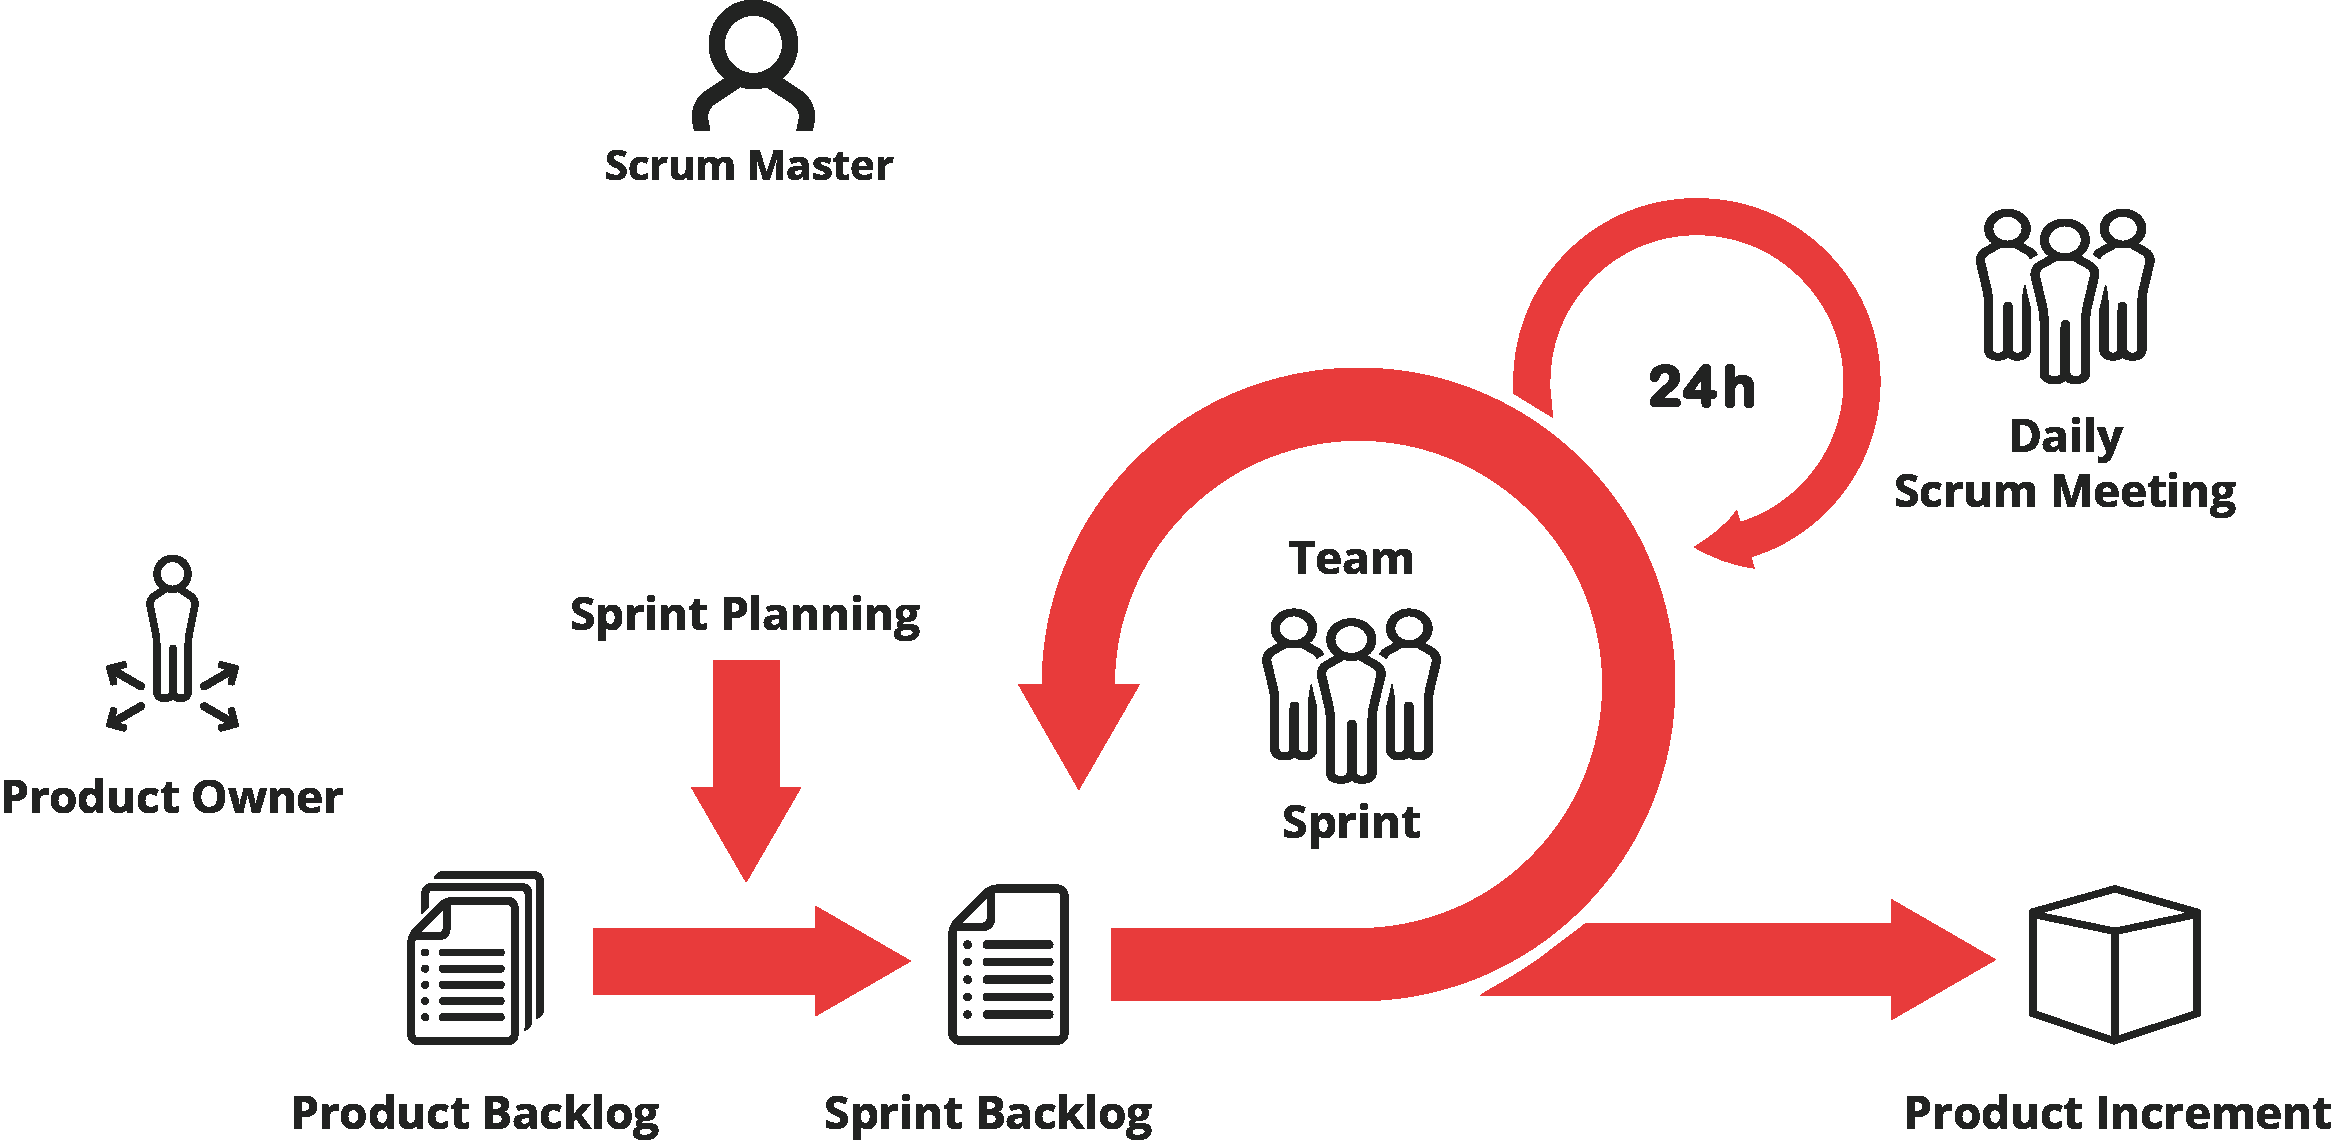
\includegraphics[width=0.8\textwidth]{pictures/scrum}
	 \caption[Agiles arbeiten mit Scrum]{Agiles arbeiten mit Scrum\cite{scrum2018}}
	 \label{fig:scrum}
\end{figure}

Die Verantwortlichkeiten liegt beim sogenannten Scrum-Team, welches sich aus folgenden Rollen ergibt:
\begin{adjustwidth}{-1in}{-1in}% adjust the L and R margins by -1 inch
	\begin{center}
		\begin{tabular}{ ccc }
			\toprule
			{Rolle} & {Besetzung in unserem Projekt} & {Anmerkung}\\

			\midrule
			{Product Owner} & {HTW Berlin} & {Vertreten durch Prod. Dr. Thomas Scheffler}\\
			{Scrum Master} & {-} & {-}\\
			{Projektmanager} & {Sidney Göhler} & {-}\\
			{Scrum Team} & {Sidney Göhler, Ilja Buschujew} & {-}\\
			\bottomrule
		\end{tabular}
		\captionof{table}{Verantwortlichen im Scrum-Team} \label{tab:scrumverantwortung} 
    \end{center}
\end{adjustwidth}


\newpage

\subsection{Projektstruktur} \label{Projektstruktur}

Aus den uns gesetzten Pflichten, haben sich für uns die folgende Projektstruktur grob herauskristalisiert, welche im laufenden Prozess immer weiter in Arbeitspakete verfeinert wurde.


\begin{center}
	\begin{figure}[h]
		 \noindent\makebox[\textwidth]{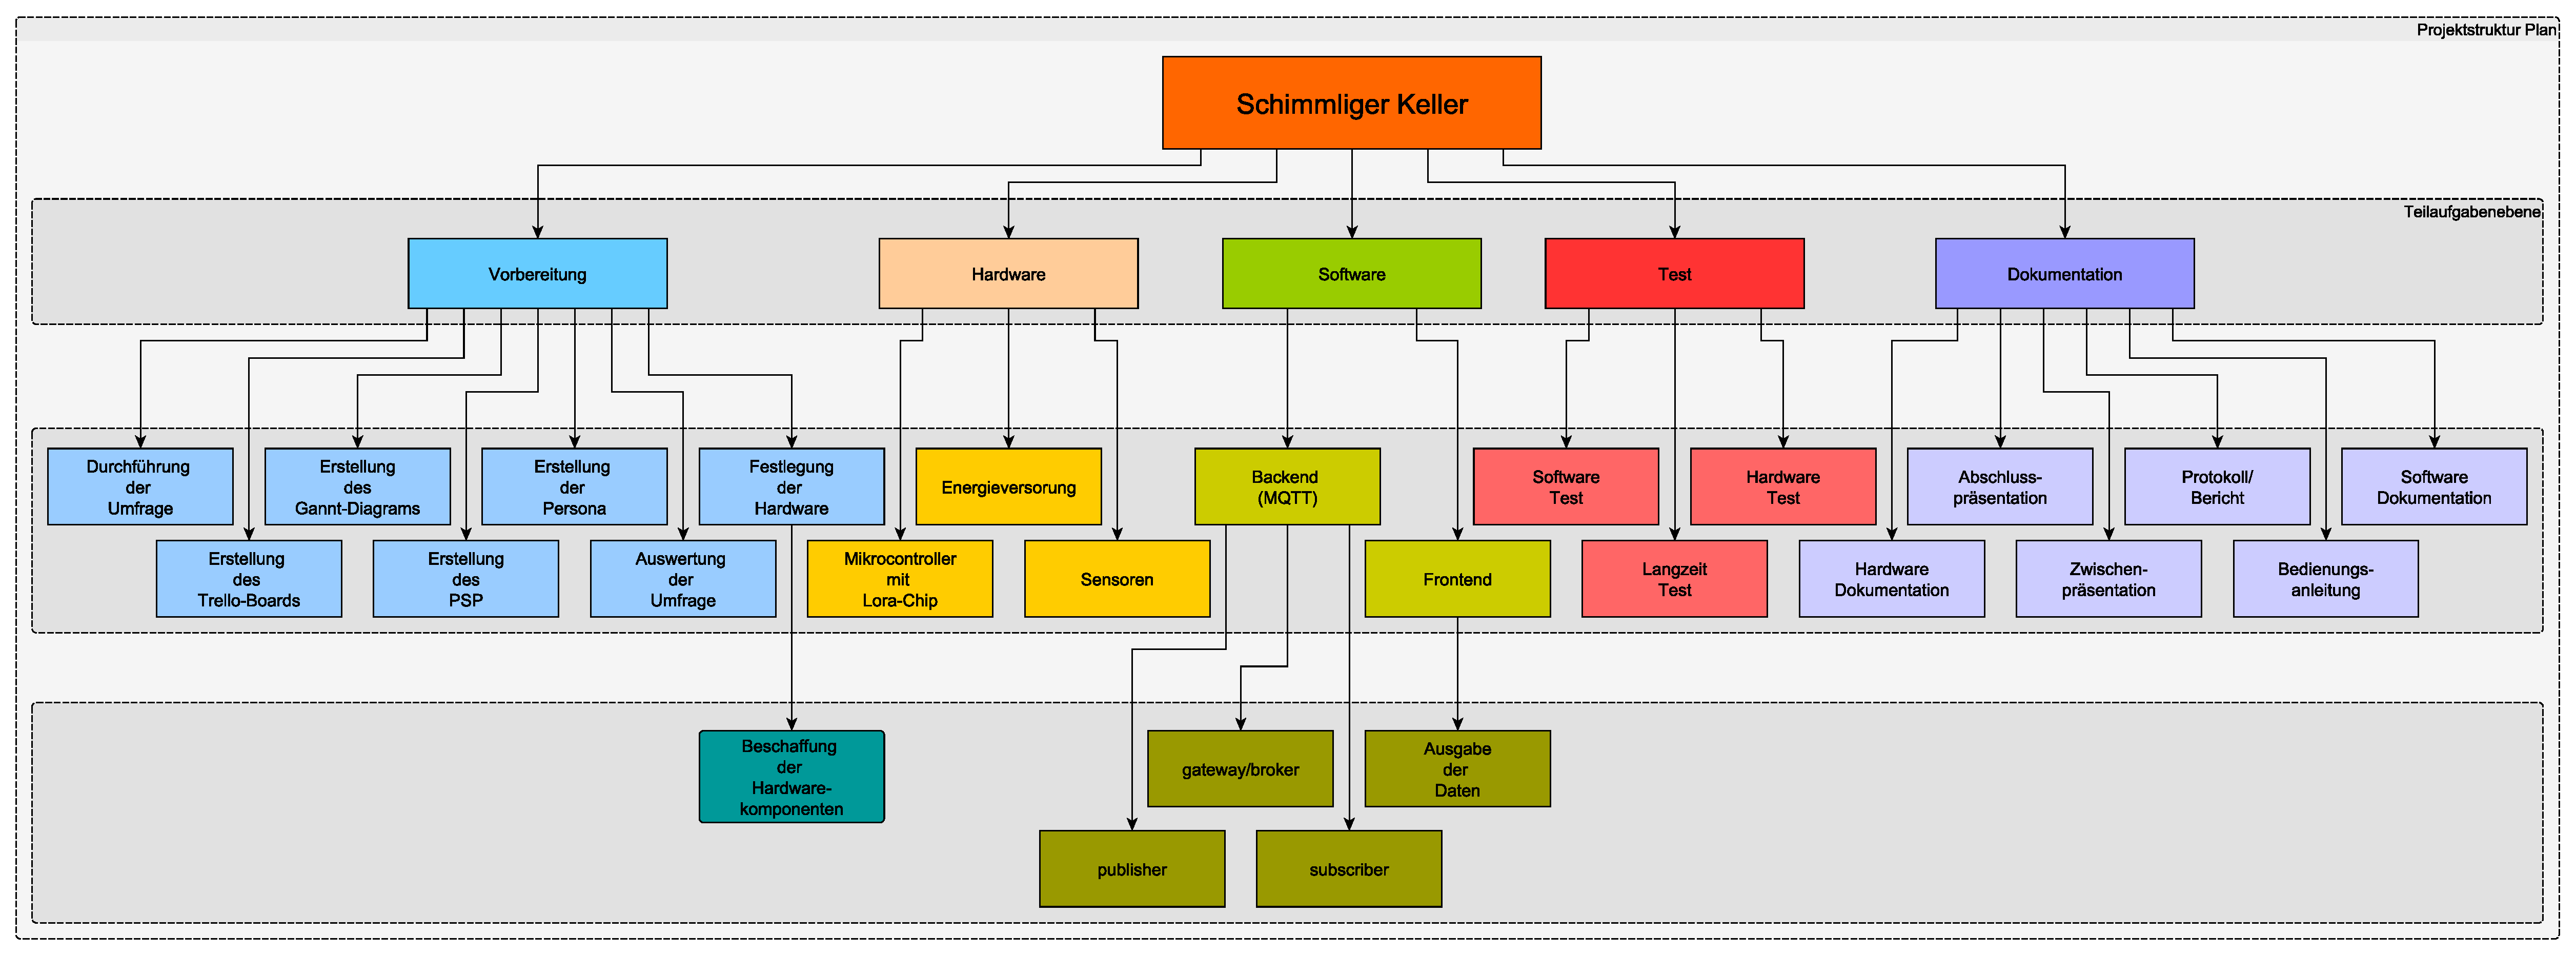
\includegraphics[width=1.2\textwidth]{pictures/PSP}}
		 \caption[Projektstrukturplan]{Projektstrukturplan} 

	\end{figure}
\end{center}

Mithilfe des Projektstrukturplanes ließen grob die einzelnen Arbeitspakete ableiten, wobei diese sich, wie bereits erwähnt, immer weiter verfeinert haben. Der enstehende Aufwand ließ sich zu Beginn noch nicht richtig abschätzen, dennoch konnten wir einen groben Zeitplan für die einzelnen Meilensteine abschätzen.

\newpage

\subsection{Zeitplanung} \label{Zeitplanung}

\begin{center}
	\begin{figure}[h]

	 \noindent\makebox[\textwidth]{
\includegraphics[width=1.3\textwidth]{pictures/zeitplanung}}
	 \caption[Übersicht unserer Zeitplanung]{Übersicht unserer Zeitplanung}
	 \label{fig:zeitplanung}
	\end{figure}
\end{center}

Illustriert wird unsere grobe Zeitplanung zu Beginn des Projektes. Wir wollten aufgrund unserer agilen Arbeitsweise nur grobe Zeiträume definieren. Wie sich schlussendlich herausgestellt hat, haben manche Teilaspekte länger, andere wiederum kürzer gerdauert.\\



\newpage
<<<<<<< HEAD
Nachfolgend wird eine tabellarische Übersicht unserer Zeitplanung aufgeführt, wobei wir die Daten aus unserem Trello-Board entnehmen:
% \begin{adjustwidth}{-1in}{-1in}% adjust the L and R margins by -1 inch
% 	\begin{center}
% 		\begin{tabular}{ ccccc }
% 			\toprule
% 			{Vorgangsname} & {Anfang} & {Ende} & {Bearbeiter} & {Arbeitszeit}\\
% 			
% 			\midrule
% 			\multicolumn{5}{c}{\textbf{Vorbereitung}} \\
% 			{Sichtung der Quellenlage} & {01.10.2021} & {20.02.2022} & S + I & 20h\\
% 			{Erstellung Trelloboard} & {01.10.2021} & {01.10.2021} & S & 30m\\
% 			{Erstellung eines Git repositories} & {01.10.2021} & {01.10.2021} & S & 30m\\
% 			{Erstellung des PSP} & {01.10.2021} & {20.02.2022} & I & 2h\\
% 			{Erstellung Zeitplan} & {01.10.2021} & {20.02.2022} & S & 2h\\
% 			{Erstellung/Durchführung der Umfrage} & {01.10.2021} & {02.12.2021} & S + I & 20h\\
% 			{Festlegung/Beschaffung der Hardware} & {01.10.2021} & {20.02.2022} & S + I & 20h\\
% 			{Auswahl/Einrichtung Software IDE} & {01.10.2021} & {20.02.2022} & S + I & 20h\\
% 			{Auswertung der Umfrage} & {01.10.2021} & {20.02.2022} & S + I & 20h\\
% 			{Erstellung des Persona} & {01.10.2021} & {20.02.2022} & S + I & 20h\\
% 
% 			\midrule
% 			\multicolumn{5}{c}{\textbf{Hardware}} \\
% 			{Inbetriebnahme der Hardware} & {01.10.2021} & {20.02.2022} & S + I & 20h\\
% 
% 			\midrule
% 			\multicolumn{5}{c}{\textbf{Software}} \\
% 			{µC Management} & {01.10.2021} & {20.02.2022} & S + I & 20h\\
% 			{Integration der Sensoren} & {01.10.2021} & {20.02.2022} & S + I & 20h\\
% 			{Einrichtung einer P2P LoRa-Kommunikation} & {01.10.2021} & {20.02.2022} & S + I & 20h\\
% 			{Entwicklung eines MQTT Publishers} & {01.10.2021} & {20.02.2022} & S + I & 20h\\
% 			{Entwicklung eines MQTT Subscribers} & {01.10.2021} & {20.02.2022} & S + I & 20h\\
% 			{Einrichtung einer grafischen Schnittstelle} & {01.10.2021} & {20.02.2022} & S + I & 20h\\
% 			{Softwaretests} & {01.10.2021} & {20.02.2022} & S + I & 20h\\
% 
% 			\midrule
% 			\multicolumn{5}{c}{\textbf{Nachbereitung}} \\
% 			{Vorbereitung der Zwischenpräsentation} & {01.10.2021} & {20.02.2022} & S + I & 20h\\
% 			{Vorbereitung der Abschlusspräsentation} & {01.10.2021} & {20.02.2022} & S + I & 20h\\
% 			{Dokumentation} & {01.10.2021} & {20.02.2022} & S + I & 20h\\
% 			{Langzeittests} & {01.10.2021} & {20.02.2022} & S + I & 20h\\
% 
% 			\bottomrule
% 		\end{tabular}
% 		\captionof{table}{Übersicht der Arbeitspakete und Arbeitszeiten} \label{tab:worklog} 
% 	\end{center}
% 
% \end{adjustwidth}
=======
Nachfolgend wird eine tabellarische Übersicht unserer Zeitplanung aufgeführt, wobei wir die Daten aus unserem Trello-Board entnehmen:\\

\begin{adjustwidth}{-1in}{-1in}% adjust the L and R margins by -1 inch
	\begin{center}
		\begin{tabular}{ ccccc }
			\toprule
			{Vorgangsname} & {Anfang} & {Ende} & {Bearbeiter} & {Arbeitszeit}\\

			\midrule
			\multicolumn{5}{c}{\textbf{Vorbereitung}} \\
			{Sichtung der Quellenlage} & {22.10.2021} & {11.02.2022} & S + I & 20h\\
			{Erstellung Trelloboard} & {22.10.2021} & {22.10.2021} & S & 30m\\
			{Erstellung eines Git repositories} & {22.10.2021} & {22.10.2021} & S & 30m\\
			{Erstellung des PSP} & {29.10.2021} & {29.02.2022} & I & 2h\\
			{Erstellung Zeitplan} & {01.11.2021} & {04.11.2022} & S & 2h\\
			{Erstellung/Durchführung der Umfrage} & {05.11.2021} & {05.11.2021} & S + I & 2h\\
			{Festlegung/Beschaffung der Hardware} & {15.11.2021} & {01.12.2021} & S + I & 3h\\
			{Auswahl/Einrichtung Software IDE} & {01.12.2021} & {20.12.2021} & S + I & 2h\\
			{Auswertung der Umfrage} & {15.11.2021} & {15.11.2021} & S + I & 1h\\
			{Erstellung des Persona} & {15.11.2021} & {15.11.2021} & S + I & 2h\\

			\midrule
			\multicolumn{5}{c}{\textbf{Hardware}} \\
			{Inbetriebnahme der Hardware} & {01.12.2021} & {27.12.2021} & S + I & 2h\\

			\midrule
			\multicolumn{5}{c}{\textbf{Software}} \\
			{µC Management} & {03.01.2022} & {10.01.2022} & S + I & 2h\\
			{Integration der Sensoren} & {10.01.2022} & {04.02.2022} & S & 6h\\
			{Einrichtung einer P2P LoRa-Kommunikation} & {17.01.2022} & {11.02.2022} & S & 6h\\
			{Entwicklung eines MQTT Publishers} & {17.01.2022} & {11.02.2022} & S + I & 2h\\
			{Entwicklung eines MQTT Subscribers} & {17.01.2022} & {11.02.2022} & S + I & 1h\\
			{Einrichtung einer grafischen Schnittstelle} & {10.01.2022} & {11.02.2022} &  I & 2h\\
			{Softwaretests und Bugfixes} & {01.10.2021} & {20.02.2022} & S + I & 6h\\

			\midrule
			\multicolumn{5}{c}{\textbf{Nachbereitung}} \\
			{Vorbereitung der Zwischenpräsentation} & {16.12.2021} & {17.12.2021} & S & 3h\\
			{Vorbereitung der Abschlusspräsentation} & {01.02.2022} & {11.02.2022} & S + I & 6h\\
			{Dokumentation} & {14.02.2022} & {25.02.2022} & S + I & 8h\\
			{Langzeittests} & {20.01.2022} & {11.02.2022} & S + I & 2h\\

			\midrule
			{\textbf{Summe}} & & & & 81h\\

			\bottomrule
		\end{tabular}
		\captionof{table}{Übersicht der Arbeitspakete und Arbeitszeiten} \label{tab:worklog} 
	\end{center}

\end{adjustwidth}
>>>>>>> baa7d21123956ad552f736e3f4632aba95a834ca

\newpage

\subsection{Kostenaufstellung} \label{Kostenaufstellung}

Auch wenn wir unser Projekt in erster Linie als Freie Software bereitstellen wollen
Aus unseren Anforderungen geht hervor, dass die meisten potentiellen Nutzer möglichst wenig für unser Produkt bezahlen möchten. Wie bei 

\begin{adjustwidth}{-1in}{-1in}% adjust the L and R margins by -1 inch
	\begin{center}

	        \begin{tabular}{cccccc}
			\toprule
			\multicolumn{3}{c}{\textbf{PyCom}} & \multicolumn{3}{c}{\textbf{DIY}}\\

			Name & Anzahl & Kosten & Name & Anzahl & Kosten\\

			\midrule
			LoPy4 & 2 & 38,45 € & ESP32 DevKit & 1 & 9,99 €\\
			Pytrack  & 1 & 40,65 € & Breadboard & 1 & 5,99 €\\
			Antennen-Kit  & 1 & 9,00 € & LoRa Transceiver + Antenne & 1 & 11,98 €\\
			Batterie-Halterung & 1 & 9,00 € & Batterie-Halterung & 1 & 9,00 € \\
			DHT22 Sensor & 1 & 9,99 € & DHT22 Sensor & 1 & 9,99 €\\
			 &  &  & Passive Bauelemente &  & 2,00 €\\

			\midrule
			\textbf{Gesamtkosten} & & 145,54 € & \textbf{Gesamtkosten} & & 48,95 €\\

			\bottomrule

	        \end{tabular}
		\label{}
		\captionof{table}{Kostenaufstellung für das Projekt} \label{tab:kostenaustellung} 
	\end{center}
\end{adjustwidth}

Anzumerken ist hier, dass die Entwicklung des Produktes mithilfe der PyCom Plattfrom zwar deutlich kostenintensiver ist, aber besonders für einen Prototypen doch recht komfortabel, da jeder einzelne Baustein dafür gemacht ist, miteinander zu funktionieren.\\
Tendenziell ließe sich aber mit einem \"Selbstbau\" der Preis um knapp die hälfte reduzieren.\\
Neben der PyCom Plattform existieren noch andere Entwicklungsplattformen, wie z.B. das \textit{TOOGOO WiFi ESP-32 Entwicklungs Board}, welches den LoRa Transreceiver implementiert und teilweise auch schon eine Halterung für Batterien anbietet.\\
Anzumerken ist auch, das der zweite LoPy4 entfallen würde, wenn man sich direkt mittels LoRaWAN an einem Gateway anmeldet und nicht wie wir es gemacht haben, zwei Microcontroller miteinander kommunizieren zu lassen.\\

\newpage


\section{Systemkonzept und theoretische Realisierung} \label{Systemkonzept und theoretische Realisierung}

Nachfolgend wird das Systemkozept und die Realisierung für unser Projekt „Luftfeuchtigkeits-Sensornetzwerk zur zeitnahen Detektion von Wasserschäden auf Basis von LoRa(WAN)“ in Form eines Blockschaltbildes beschrieben. 

\begin{figure}[h]
 \centering
 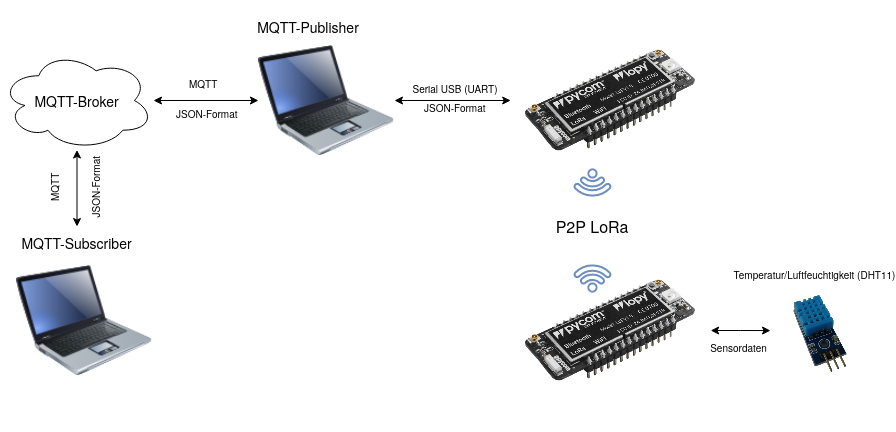
\includegraphics[width=1\textwidth]{pictures/Blockschaltbild_ProNeSy}
 \caption[Systemkonzept für unser Projekt]{Systemkonzept für unser Projekt}
 \label{fig:systemkonzept}
\end{figure}

Für unser Projekt haben wir uns, nach der Beratung mit Prof. Scheffler, dafür entschieden mit den Pycom-Entwicklungsboards zu arbeiten. Diese Boards haben den Vorteil, dass dort schon ein LoRa-Transceiver-Chip integriert ist. 

Da nun sich ein Board mit dem Sensor für die Ausmessung der Luftfeuchtigkeit im Keller befinden soll, wird das andere Board dafür benötigt, um die Sensordaten über LoRa-Kommunikation, in einem Bereich wo es eine Internetverbindung gibt, zu empfangen und über das MQTT-Protokoll an den MQTT-Broker weiterzuleiten, damit andere, die an den Sensordaten interessiert sind, darauf zugreifen können. Als Datenformat wurde sowohl für die Übertragung mittels LoRa, als auch MQTT, JSON verwendet.

Zur Weiterleitung der Sensordaten an den MQTT-Broker wurden die von dem Board empfangenen Sensordaten mithilfe einer UART-Verbindung am Computer ausgelesen und in Form eines Publisher-Clients versendet. Der Subscriber-Client kann nun die jeweiligen Sensorwerte auf den jeweiligen Topics, die er einsehen möchte, empfangen.

Für die Visualisierung der Sensordaten haben wir uns für die Adafruit IO Plattform entschieden\footnote{https://io.adafruit.com/}. Diese Plattform bietet abgesehen von den tollen Visualisierungen der Sensorwerte im Form eines Dashboards, auch einen MQTT-Broker an, den man mit einigen bestimmten Einschränkungen bei der kostenlosen Variante für die eigene Anwendung nutzen kann. 
<<<<<<< HEAD
=======

\begin{figure}[h]
	 \centering
	 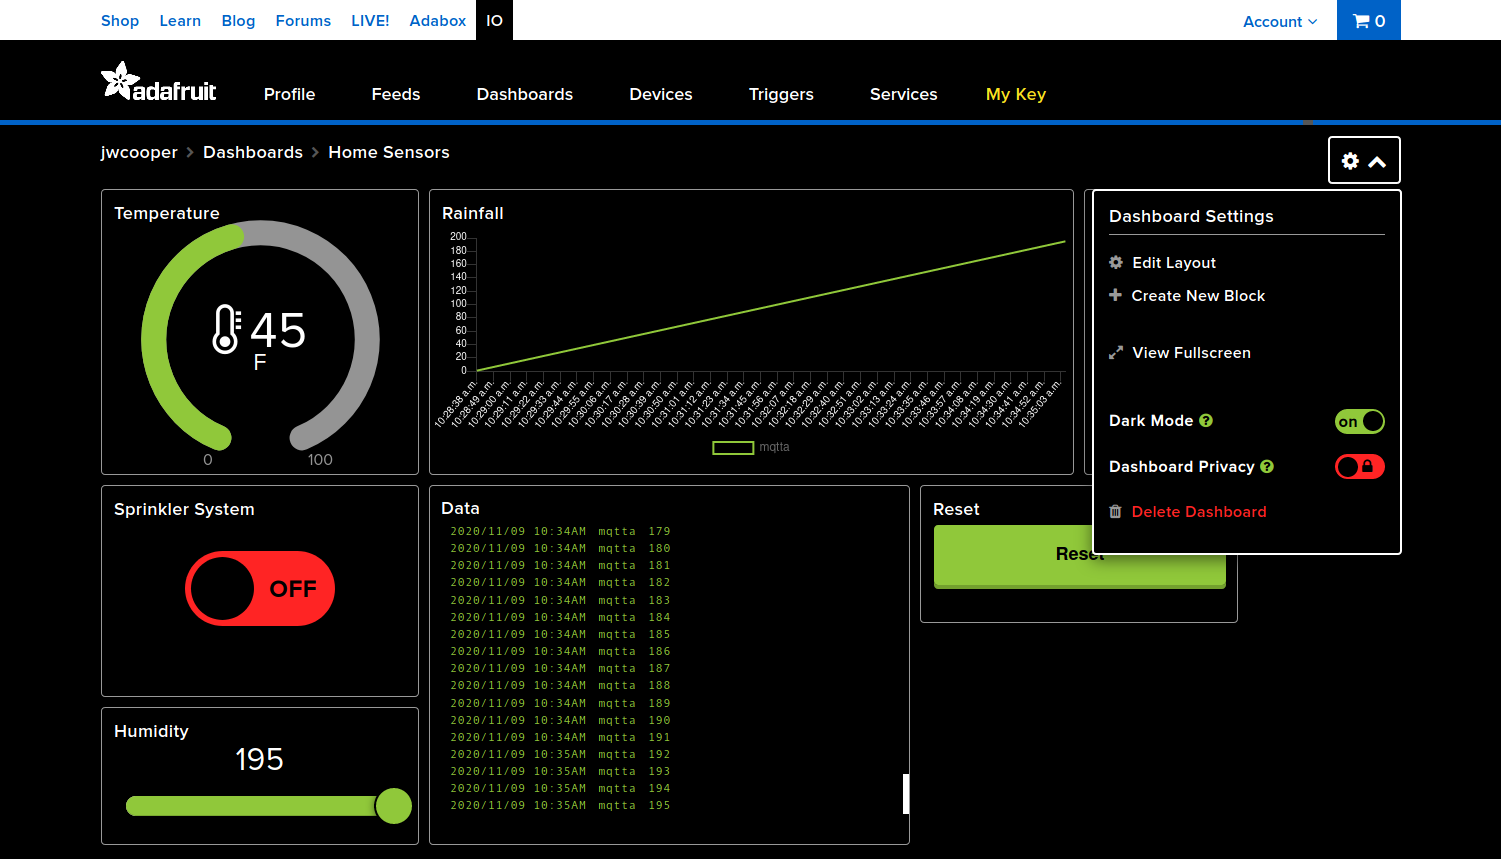
\includegraphics[width=0.8\textwidth]{pictures/adafruitdashboard}
	 \caption[Beispielhaftes Adafruit Dashboard]{Beispielhaftes Adafruit Dashboard\cite{adafruitdash}}
	 \label{fig:adafruitdashboard}
\end{figure}
>>>>>>> baa7d21123956ad552f736e3f4632aba95a834ca

% !TEX root = ../Thesis.tex
%%
%%  Hochschule für Technik und Wirtschaft Berlin --  Projektabschlussbericht
%%
%% Kapitel 3 - Grundlagen
%%
%%

\chapter{Grundlagen} \label{Grundlagen}
\section{LoRa und LoRaWAN} \label{LoRa und LoRaWAN}
\subsection{LoRa} \label{LoRa}

Der Begriff LoRa steht für \textbf{L}ong \textbf{R}ange und definiert dabei ein für weite Strecken ausgelegtes, funkbasiertes Übertragungsverfahren auf der Bitübertragungsschicht (physical layer) im OSI-Schichtenmodell. Es wurde von Nicolas Sornin und Olivier Seller in deren französischen Firma Cycleo, welche später von Semtech Corporation abgekauft wurde, im Jahr 2009 entwickelt \cite{semtech2020}. 

LoRa kann zu den sogenannten \textbf{L}ow-\textbf{P}ower-\textbf{W}ide-\textbf{A}rea-\textbf{N}etwork (LPWAN) Technologien zugeordnet werden, die einen energiesparsamen Betrieb und eine hohe Übertragunsreichweite aufweisen. Im Vergleich zu WLAN oder Mobilfunk, fällt jedoch die Daten- bzw. Bandbreite bei diesen Technologien relativ gering aus, sodass diese hauptsächlich bei drahtlosen Sensornetzwerken Anwendung finden, wo es darum geht Sensordaten mit einer geringen Datenrate über eine weite Funkstrecke zu übertragen. Ein Vergleich zu den funkbasierten Technologien (WLAN, LPWAN und Mobilfunk) stellt die Abb. \ref{fig:lpwan} dar.

\begin{figure}[h]
 \centering
 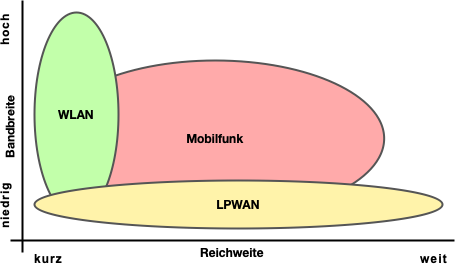
\includegraphics[width=0.7\textwidth]{pictures/lpwan-wlan-mobilfunk}
 \caption[Vergleich zwischen WLAN, Mobilfunk und LPWAN bezüglich der Bandbreite und Reichweite]{Vergleich zwischen WLAN, Mobilfunk und LPWAN bezüglich der Bandbreite und Reichweite \cite{lpwan2022}}
 \label{fig:lpwan}
\end{figure}

Die hohe Reichweite, bei gleichzeitig energiesparsamem Betrieb, erzielen die LPWAN Technologien mithilfe von Frequenzen unterhalb des 1 GHz Bereiches. Da LoRa ebenfalls zu den LPWAN Technologien zählt, nutzt diese in Europa die lizenfreien 433 und 868 MHz ISM-Frequenzbänder. Die Frequenzbänder unterscheiden sich jenach Land und Region auf der ganzen Welt. In den USA z.B. liegt der nutzbare Frequenzband bei 915 MHz. Das 433 MHz Frequenzband ist jedoch nur für unidirektionale Übertragung, wo man entweder nur Senden oder Empfangen kann, vorgesehen. Hingegen ist das 868 MHz Band bidirektional, das heißt, dass damit das gleichzeitige Senden und Empfangen gewährleistet ist \cite{lpwan2022}. 

Die jeweiligen Frequenzbänder haben eine bestimmte Frequenzbandbreite und werden wiederum in sogenannte Funkkanäle unterteilt, mit einer bestimmten Kanalbandbreite, um das gegenseitige stören gleicher Frequenzen zu minimieren. So weist z.B. das 868 MHz Frequenzband eine Frequenzbandbreite zwischen 863 und 870 MHz auf \cite{Staniec2020}. So können benachbarte Funkknoten, die sich im gleichen 868 MHz Frequenzband befinden, aber einen unterschiedlichen Funkkanal nutzen, gleichzeitig senden und empfangen, ohne sich dabei zu stören. 

Darüberhinaus werden weitere regulatorische Maßnahmen ergriffen, wie die Festlegung einer Zeit in Form eines \textbf{D}uty-\textbf{C}ycles (DC), welches angibt, wie lange ein Funkknoten auf das Medium pro Tag zugreifen darf. Dieser ist ein prozentualer Wert und liegt bei LoRa normalerweise bei 1\% oder 10\% je nach Funkkanal und Sendeleistung \cite{Staniec2020}. 

Die Abbildung \ref{fig:868-band} zeigt das 868 MHz-Frequenzband mit den jeweiligen Funkkanälen, deren Bandbreite (in kHz), der äquivalenten Strahlungsleistung (in dBm) und des jeweiligen Duty Cycles an . 

\begin{figure}[h]
 \centering
 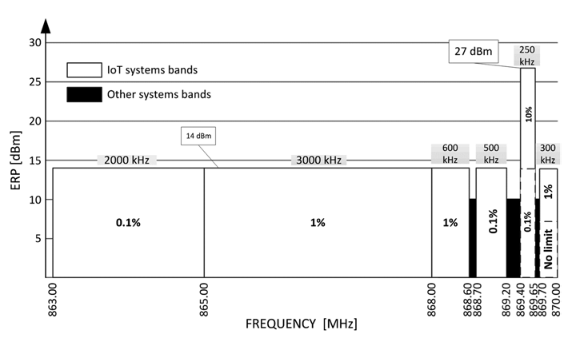
\includegraphics[width=0.9\textwidth]{pictures/868-band}
 \caption[Aufteilung des 868-ISM-Bandes in Funkkanäle nach ETSI EN 300 220-2]{Aufteilung des 868-ISM-Bandes in Funkkanäle nach ETSI EN 300 220-2 \cite{Staniec2020}}
 \label{fig:868-band}
\end{figure}

Weitere Möglichkeiten zur Verhinderung der gegenseitigen Störung, sind die definierten Zugriffsverfahren auf das Medium, die bei LPWAN auch als \textbf{P}olite-\textbf{M}edium-\textbf{A}ccess (PMA) heißen. Darunter zählt das sogenannte \textbf{C}lear-\textbf{C}hannel-\textbf{A}ssessment (CCA), welches wiederum in \textbf{A}daptive-\textbf{F}requency-\textbf{A}gility (AFA) und \textbf{L}isten-\textbf{B}efore-\textbf{T}alk (LBT) eingeteilt werden kann. Dabei ähnelt das CCA-Zugriffsverfahren sehr stark dem Carrier-Sense-Multiple-Access/Collision-Avoidance (CSMA/CA) Zugriffsverfahren bei z.B. WLAN.

Bei dem AFA Verfahren, wird einerseits die Datenrate hinsichtlich der Kanaleigenschaften angespasst und andererseits ein geeigneter Funkkanal mittels spezieller Algorithmen, die die optimale Lastverteilung zwischen den jeweiligen Funkkanälen berechnen, ausgewählt. Das LBT Verfahren stellt sicher, dass immer nur ein Funkgerät auf einen Funkkanal zugreifen kann, um die gegenseitige Störung zu verhindern. So „lauscht“ (listen) es zunächst einmal auf den Funkkanal, auf dem es zugreifen möchte, um festzustellen ob es frei ist, bevor es darauf zu „sprechen“ (talk) beginnt. Wenn das Funkgerät feststellt, dass der Kanal momentan besetzt ist, dann wartet es eine gewisse Zeit, die normalerweise zwischen 5 und 10 ms beträgt, ab, bevor es nochmal versucht auf den Kanal zuzugreifen \cite{Staniec2020}. 

Die Reichweite von LoRa beträgt zwischen 2-5 km in urbanen und 5-15 km in ländlichen Regionen mit keiner direkten Sichtverbindung (non-line-of-sight). Wenn es eine direkte Sichtverbindung (line-of-sight) zwischen den Funkmasten gibt, dann kann die Reichweite auch weit über 15 km erreichen. LoRa hat zudem eine sehr gute Gebäudedurchdringung, was es zu einer idealen Technologie für den Einsatz in Kellern ausmacht. Die Datenrate liegt dabei im Bereich zwischen 0.3 kBit/s  und 5.5 kBit/s und die maximale Übertragungsleistung bei 25 mW \cite{lora2022}. Der aktuelle Rekord, bei dem die Sensorwerte noch empfangen konnten, liegt bei einer unglaublichen Reichweite von 766 km, welcher im Juli 2019 aufgestellt wurde\footnote{https://tech-journal.semtech.com/university-of-zaragoza-breaks-long-range-lorawan-based-signal-record}.

Die hohe Reichweite, bei gleichzeitig geringem Energieverbrauch, ist abgesehen von der niedrigen Frequenz, dem speziellen Modulationssverfahren zu verdanken. LoRa benutzt die sogenannte \textbf{C}hirp-\textbf{S}pread-\textbf{S}pectrum (CSS) Modulationstechnik, bei der sich die Frequenz eines Signals (0 oder 1) innerhalb eines definierten Frequenzbereiches gleichmäßig ändert (siehe Abb. \ref{fig:css}). Dieses Modulationsverfahren existierte schon vor der Erfindung von LoRa und zwar bei der Unterwasserkommunikation und den Sonargeräten im maritimen Sektor, sowie der Radartechnologie in der Luftfahrt \cite{semtech2020}.

\begin{figure}[h]
 \centering
 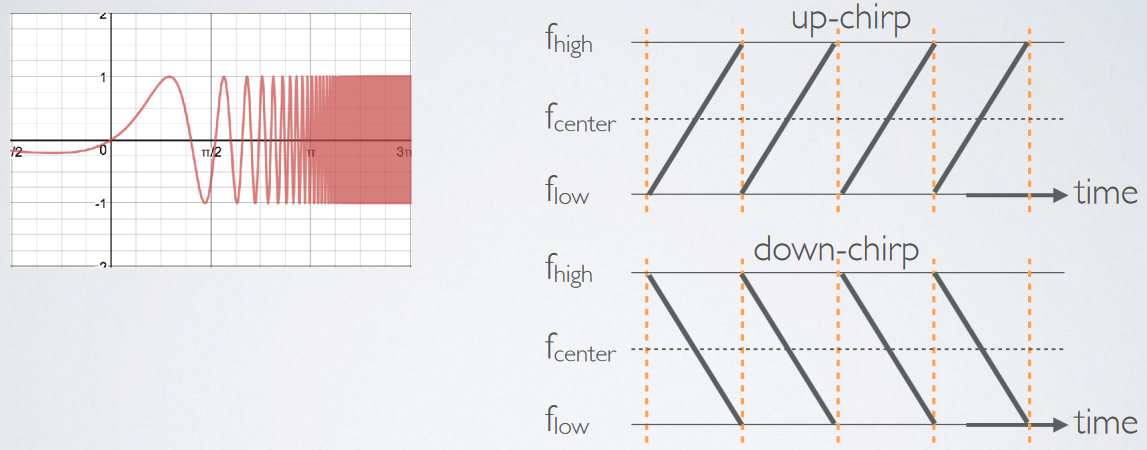
\includegraphics[width=0.9\textwidth]{pictures/chirp-sf}
 \caption[chirp spread spectrum]{chirp spread spectrum \cite{lora2022}}
 \label{fig:css}
\end{figure}

Die gleichmäßige Änderung der Frequenz innerhalb eines definierten Frequenzbereiches wird als chirp (zwitschern oder zirpen) bezeichnet und ist in der Natur weit verbreitet. So kommunizieren z.B. Vögel, Fledermäuse oder Delphine ebenfalls über die zeitliche Änderung der Frequenz. Dies hat den Vorteil, dass äußere Störungen einen geringeren Einfluss auf die Signalqualität ausüben und somit das Signal-Rausch-Verhältnis sich verbessert. Außerdem ist das CSS Verfahren weniger anfällig gegenüber den sogenannten Doppler-Effekt, bei dem es zu Signalverzerrungen bei dem Empfänger, wenn der Sender oder Empfänger in Bewegung sind, kommt. 

Durch das hinzufügen eines sogenannten Spreizfaktors (Spreading Factor oder SF), kann außerdem die Geschwindigkeit der zeitlichen Änderung der Frequenz, also die Chirprate geändert und damit auch die Datenrate variiert werden. LoRa definiert dabei insgesamt sechs Abstufungen des Spreizfaktors (SF6 bis inkl. SF12) \cite{sf2022}.

Grundsätzlich gilt; je kleiner der Spreizfaktor, desto höher ist die Chirprate und damit auch die Datenrate der Übertragung. Jedoch nimmt die Reichweite der Datenübertragung, je kleiner der Spreizfaktor ist, ab. Bei der Erhöhung des Spreizfaktors um einen Wert, halbiert sich die Chirprate und damit auch die Datenrate, aber die Reichweite wird erhöht. 

Auf der anderen Seite nimmt die Batterielaufzeit mit abnehmenden Spreizfaktor zu, da die Zeit, bei der das LoRa-Funkmodul zur Übertragung der Daten aktiv sein muss, aufgrund der erhöhten Chirp- bzw. Datenrate, abnimmt. 

Darüberhinaus kann durch die Erhöhung der Kanalbandbreite, bei gleichbleibenden Spreizfaktor, ebenfalls eine Erhöhung der Datenrate bewirkt werden. 

Mit der Änderung des Spreizfaktors und damit auch der Datenrate, können „Datenstaus“ im Netzwerk aktiv reguliert werden \cite{sf2022}. 

\subsection{LoRaWAN} \label{LoRaWAN}

Da LoRa anfangs nur für die Bitübertragungsschicht definiert wurde, musste ein Mechanismus entwickelt werden, bei dem die LoRa-Endgeräte addressiert untereinander und mit den LoRa-Gateways kommunizieren können. Es wurde zunächst einmal das LoRaMAC-Protokoll für die Sicherungsschicht (MAC layer) definiert. Später wurde die LoRa-Alliance\footnote{https://lora-alliance.org/} gegründet, die es zu LoRa-\textbf{W}ide-\textbf{A}rea-\textbf{N}etwork (LoRaWAN) umbenannt hat \cite{semtech2020}.

LoRaWAN nutzt für die Kommunikation zwischen den LoRa-Endgeräten und LoRa-Gateways die Sterntopologie (siehe Abb. \ref{fig:lorawan-topology}).

\begin{figure}[h]
 \centering
 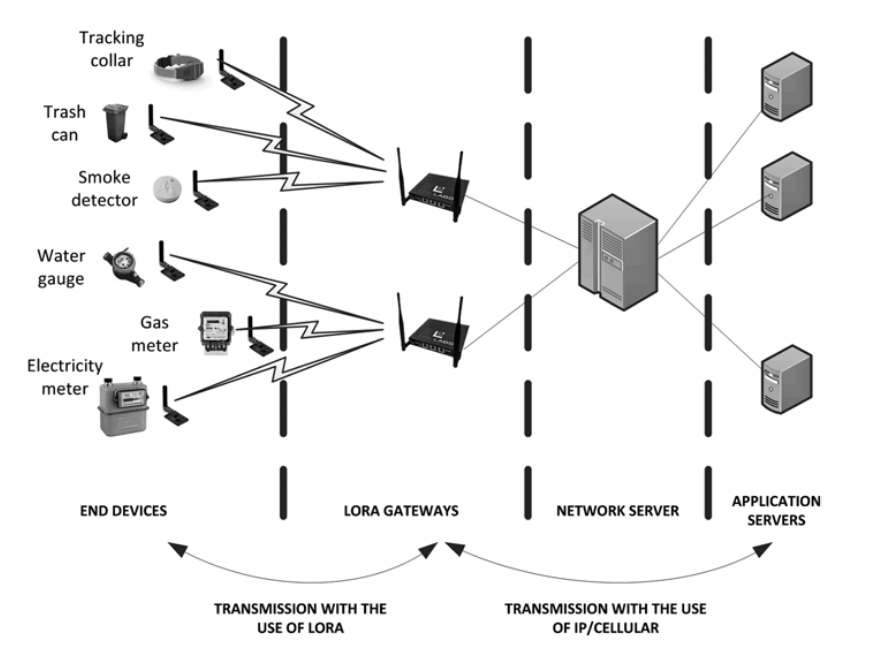
\includegraphics[width=0.9\textwidth]{pictures/lorawan-topology}
 \caption[LoRaWAN Topologie]{LoRaWAN Topologie \cite{Staniec2020}}
 \label{fig:lorawan-topology}
\end{figure}

Die LoRa-Endgeräte sammeln z.B. Sensor- und Messdaten und senden diese mithilfe von LoRa-Funktechnik an die LoRa-Gateways. 

Die LoRa-Gateways leiten die Daten dann über das Internet-Protokoll (IP), oder Mobilfunk an die Netzwerk-Server (Network Server) weiter. Es können mehrere LoRa-Gateways, die örtlich von einander getrennt sind, dazu genutzt werden, die Sensordaten der selben LoRa-Endgeräte zu empfangen. Durch die redundante Übertragung der selben Daten an mehrere Gateways, wird die Zuverlässigkeit und damit auch die Ausfallsicherheit der Datenübertragung verbessert.

Der Netzwerk-Server ist für die Entfernung der duplizierten Datenpakete, deren Dekodierung und für das Erstellen neuer Datenpakete, die an die LoRa-Endgeräte gesendet werden, zuständig. 

Schließlich verarbeiten die Anwendungs-Server (Application Server) die von den Netzwerk-Server erhaltene Daten für eigene Zwecke dann weiter. 


\section{MQTT} \label{MQTT}

\ldots



% !TEX root = ../Abschlussbericht_Schimmeliger_Keller.tex
%%
%%  Hochschule für Technik und Wirtschaft Berlin --  Projektabschlussbericht
%%
%% Kapitel 4 - Praktische Umsetzung
%%
%%

\chapter{Praktische Umsetzung} \label{Praktische Umsetzung}
\section{Verwendete Hardware} \label{Hardware}
\subsection{LoPy4-Development-Board} \label{LoPy4}

Das LoPy4 ist ein von Pycom Ltd. hergestelltes Development-Board für die Anwendungen im IoT-Bereich. Es unterstützt viele Schnittstellen und Übertragungsprotokolle, die für IoT-Anwendung von großer Relevanz sind. Die Abbildung \ref{fig:lopy-blockschaltbild} stellt die Funktionalitäten des LoPy4-Development-Boards in Form eines Blockdiagrammes  dar. 

\begin{figure}[h]
 \centering
 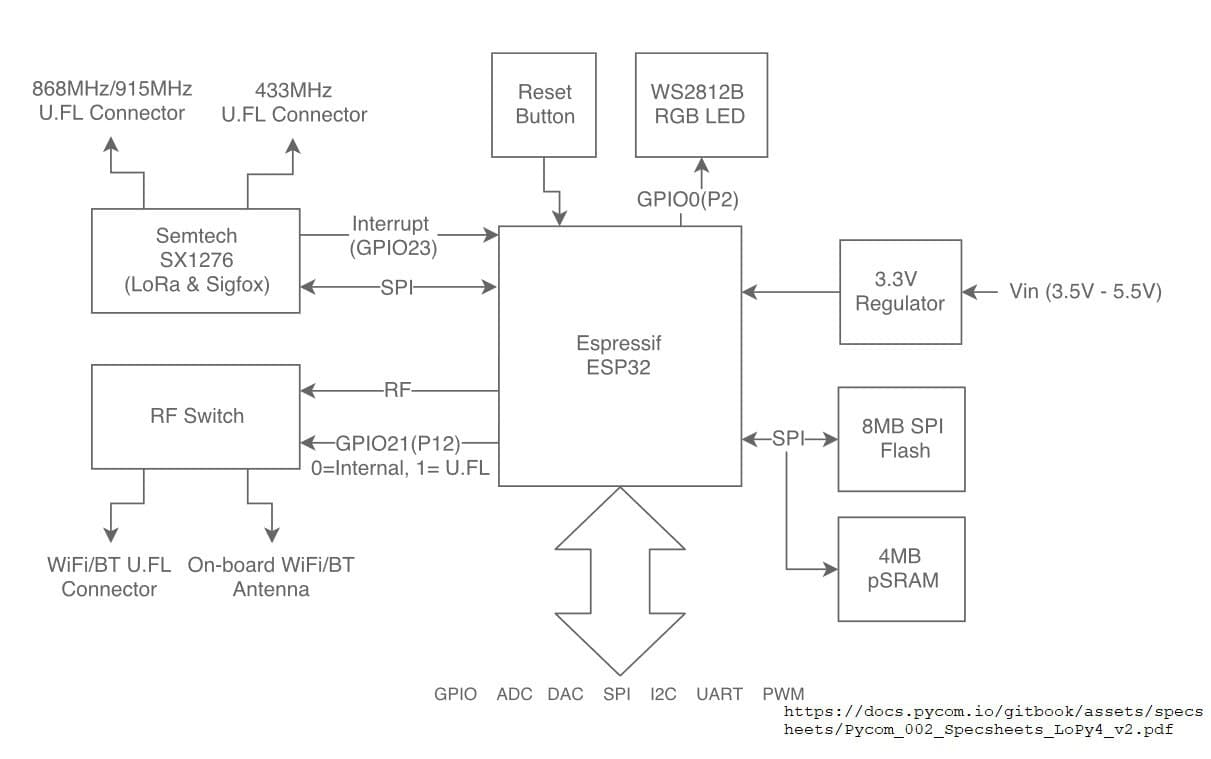
\includegraphics[width=1\textwidth]{pictures/blockdiagram_lopy}
 \caption[LoPy4-Blockdiagramm]{LoPy4-Blockdiagramm}\cite{Lopy2022}
 \label{fig:systemkonzept}
\end{figure}

Im Kern befindet sich ein Espressif ESP32 mit Xtensa dual-core-32-bit LX6 Mikroprozessor. Als Speicher verwendet es 520KB + 4MB RAM und einen externen 8MB Flash-Speicher, wohin auch der Code dann geladen wird. 
Zur Ein-/Ausgabe und der Steuerung von Sensoren und Aktoren, bietet das Board vielseitige Peripherien wie GPIO, ADC, DAC, SPI, I2C, UART und PWM an. 

Darüberhinaus verfügt das Entwicklungsboard über WLAN (802.11b/g/n/e/i), Bluetooth/Bluetooth Low Energy (BLE) v4.2, sowie LoRa und Sigfox Protokolle.  
Es lässt sich leicht mit einem Breadboard benutzen, um damit einfache Schaltungen, ohne zu löten, testen zu können. 

Für die WLAN und Bluetooth Anwendung kann man entweder die interne, im Board eingebaute, oder eine externe Antenne verwenden. Bei der Nutzung von LoRa und Sigfox muss man jedoch darauf achten, dass man unbedingt eine externe Antenne verwendet, denn sonst könnte damit der LoRa-Chip beschädigt und unbrauchbar gemacht werden. Dafür gibt es zwei Anschlussmöglichkeiten; einmal für das 868 MHz und einmal für das 433 MHz Frequenzband. 

Dafür wird der SX1276 LoRa-Transceiver-Chip der Firma Semtech verwendet.

\subsection{Mögliche Schaltung zum Selbstbauen} \label{LoPy4}

\subsection{DHT Sensormodul} \label{DHT}

Bei dem verwendeten Sensor handelt es sich um einen sog. DHT Sensor. Diesen gibt es in zwei verschiedenen Ausführungen, DHT11 und DHT22, wobei sich diese im auswertbaren Messbereich, der Messgenauigkeit und im Preis unterscheiden.

Dafür wird der SX1276 LoRa-Transceiver-Chip der Firma Semtech verwendet. 

Für die Spannungsversorgung wird lediglich ein Mikro-USB-Kabel, welches an eine USB-Schnittstelle am Computer das Board mit 3.3-5.5V versorgt, benötigt. Neben der Spannungsversorgung kann damit auch das Board direkt programmiert werden. 

Für die Programmierung des Boards kann man auf unterschiedliche Entwicklungsumgebungen zurückgreifen. So werden die Entwicklungsumgebungen wie Atom und Visual Studio Code (VSC) von dem Hersteller mit einem sogenannten Pymakr-Plugin für einen reibungslosen Upload und das Flashen des Boards unterstützt. Wenn das Benutzen des Plugins nicht möglich ist, wie unter anderem es teilweise bei uns der Fall war, so kann man auf das von PyCom angebotene File-Transfer-Protocol (FTP) zugreifen. Dafür muss man zunächst einmal einen FTP-Server auf dem Board erzeugen, mithilfe dessen man dann auf das Filesystem des Boards Zugriff hat. Damit der Code im Board läuft, muss man lediglich die jeweiligen Dateien (hauptsächlich die main.py Datei) auf das Board mit FTP-Befehlen in den Flash-Speicher kopieren. 

Für die Unterstützung von LoRa bietet es zwei Möglichkeiten: LoRa-RAW und LoRaWAN. 

Mit LoRa-RAW kann eine direkte Punkt-zu-Punkt Verbindung für die Kommunikation zwischen zwei LoRa-Knoten hergestellt werden. Mit LoRaWAN kann darüberhinaus der LoRa-Knoten in das TheThingsNetwork (TTN) oder das Chirpstack-Netzwerk eingebunden werden. Die Bandbreite kann zwischen den Werten 125, 250 und 500 kHz variiert werden. Außerdem kann man den Spreizfaktor zwischen 7 und 12 auswählen. Für die Synchronisation kann die Preamble mit der Anzahl der Chirps angepasst werden, wobei der Standardwert bei acht liegt. Wieviele „Chips” ein Symbol definieren, kann man mit der Coderate einstellen.

Darüberhinaus ist zu erwähnen, dass PyCom mit PyMesh, auch die Möglichkeit eines LoRa-Mesh-Netzwerkes auf der MAC-Ebene anbietet. Es ist dabei wichtig, dass alle LoRa-Knoten das gleiche Frequenzband, Spreizfaktor und Bandbreite verwenden. Es verwendet dazu ein hierarchisches Mesh-Netzwerkmodell.


\subsection{DHT Sensormodul} \label{DHT}

\begin{center}
	\begin{figure}[h]
	 
	 \noindent\makebox[\textwidth]{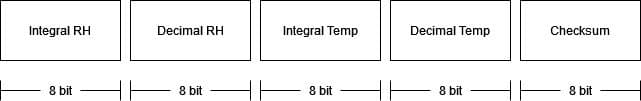
\includegraphics[width=0.7\textwidth]{pictures/dht11_dataframe}}
	 \caption[DHT Paketstruktur]{DHT Paketstruktur}
	 \label{fig:zeitplanung}
	\end{figure}
\end{center}



\subsection{Restliche Hardware} \label{Restliche Hardware}




\section{Beschreibung der Software} \label{Software}

Für unser Projekt haben wir drei verschiedene, miteinander interagierende Software Komponenten realisiert, welche über eine Schnittstelle (Interface) miteinander kommunizieren. 
Der Vorteil einer solchen Architektur ist, dass die einzelnen Komponenten sich unter umständen wiederverwenden lassen und sich im Idealfall so eine Software modular aufbauen lässt.
Da wir als Programmiersprache ausschließlich Python bzw. Micropython verwendet haben, könnte man argumentieren, dass unsere Software automatisch Modular ist, da sich in der Theorie alle programmierten Komponenten in Python wiederverwenden lassen.
Dies ist aber sehr verallgemeinert gesprochen, da gerade die Programmierung der Mikrocontroller definitiv auch Individualsoftware benötigt, welche sich aber immerhin nicht nur auf einer einzelnen Mikrocontrollerfamilie ausführen funktionieren würde.
Anzumerken ist noch, dass für unsere finale Version des Projektes vermutlich nur eine einzelne Softwarekomponente notwendig wäre.


\subsection{1. Komponente: Sensoransteuerung und der Versand der Daten mittels LoRa(WAN)} \label{Sender}

Für die Programmierung der Mikrocontroller verwenden wir die Programmiersprache Micropython, welche eine schlanke und schnelle Implementation der Programmiersprache Python ist, welche für Mikrocontroller optimiert wurde.

\begin{center}
	\begin{figure}[h]
	 
	 \noindent\makebox[\textwidth]{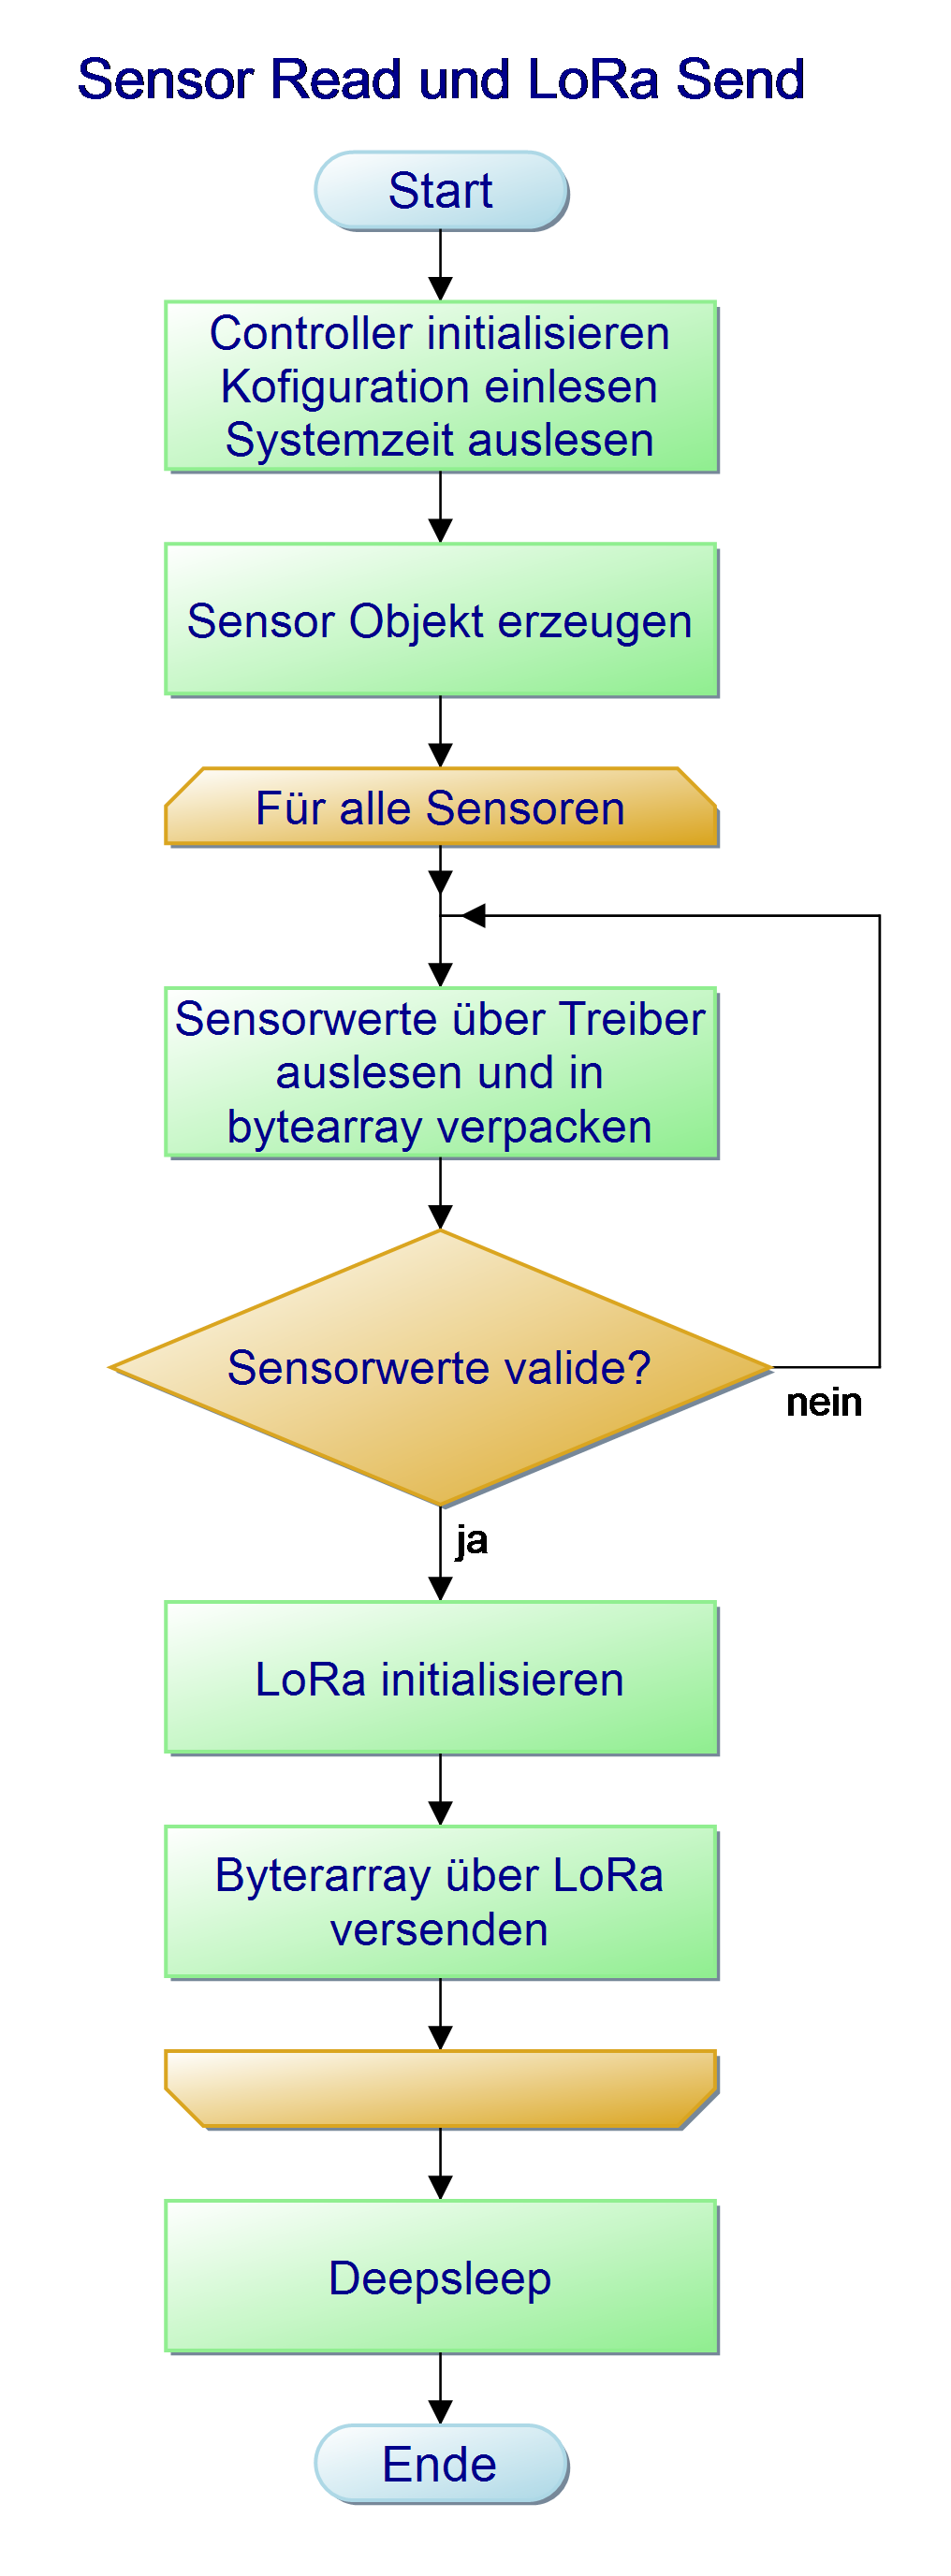
\includegraphics[width=0.4\textwidth]{pictures/sens_read_lora_send}}
	 \caption[PAP komponente 1]{Programm Ablauf: Komponente 1}
	 \label{fig:zeitplanung}
	\end{figure}
\end{center}

\subsection{2. Komponente: Emfangen der Daten und Versand ins Internet} \label{Empfänger}

\ldots
=======
Zunächst wird der Microcontroller initialisiert, wobei er standartmäßig mit allen Modulen (WiFi, LoRa, etc.) im aktivierten Zustand startet. Dieser Umstand beruht darauf, dass wir die PyCom Plattform nutzen, welche wenig vorab Konfiguration ermöglicht.\\
Jegliche Konfigurationsmöglichkeiten unserer Programme haben wir in extern Dateien im JSON Format abgelegt, welche im nächsten Schritt eingelesen werden. In der Konfigurationsdatei können unter Anderem die Dauer, die der Microcontroller im Schlafmodus verbringen soll, sowie die einzelnen Sensoren definiert werden.\\
Um das anbinden mehrere Sensonren zu ermöglichen haben wir uns dazu entschieden, eine Klasse zu programmieren, welche eben dieses Sensorobjekt darstellen soll. Der Treiber wurde von einem Benutzer auf github veröffentlicht, funktioniert aber im Prinzip nach dem oben genannten Verfahren, was bedeutet, dass zunächst eine gewisse Zeit gewartet wird, anschließend das Bus auf GND Niveau gezogen wird, um den Sensor mitzuteilen, dass er doch bitte anfängt Messwerte zu sammeln. Nachdem der Sensor eine Antwort gegeben hat, werden die empfangenen Bits zunächst alle gesammelt und anschließend in 5 einzelne Bytepakete decodiert. Abschließend prüft der Treiber mithilfer der Prüfsumme, ob die empfangenen Daten Sinn machen.\\ Je nach Sensortyp (DHT11/22) werden die empfangenen Daten nochmals in den richtigen Wertebereich \grqq verschoben\grqq.\\
Anschließend werden für alle initialisierten Sensoren, über den Treiber die aktuellen Messwerte eingelesen und in ein bytearray verpackt, wobei hier schon das erste mal geschaut wird, ob die gemessen Sensorwerte überhaupt Sinn ergeben bzw. in dem vom Hersteller angebenen Bereich fallen, da es selbst bei der korrekten Dekodierung immernoch zu unsinnigen Werten kommen kann. 
Wurde dieser Test erfolgreich bestanden wird im Microcontroller über das LoRa Modul über eine Bibliothek initialisiert und die ermittelten Werte werden versendet.\\ Ein weiterer Bestandteil des bytearrays ist die aktuelle Systemzeit, welche verwendet wird, um im späteren Verlauf ermitteln zu können, ob es sich wirklich um ein neues empfangenes Datenpaket handelt, oder ob das Paket in irgendeinem Puffer zunächst verloren gegangen ist und zufällig wieder ins Tageslicht gerückt ist.\\
Zu guter Letzt wird der Microcontroller in den Schlafmodus versetzt, wobei die Zeit, die er im stromsparenden Modus verbringt benutzerdefiniert ist. Die Systemzeit läuft auch im Schlafmodus weiter, solange der Microcontroller mit Strom versorgt wird, nur das LoRa-Modul muss neu initialisiert werden.\\

\newpage

\subsection{2. Komponente: Emfangen der Daten und Versand ins Internet} \label{Empfänger}

\begin{center}
	\begin{figure}[h]
	 
	 \noindent\makebox[\textwidth]{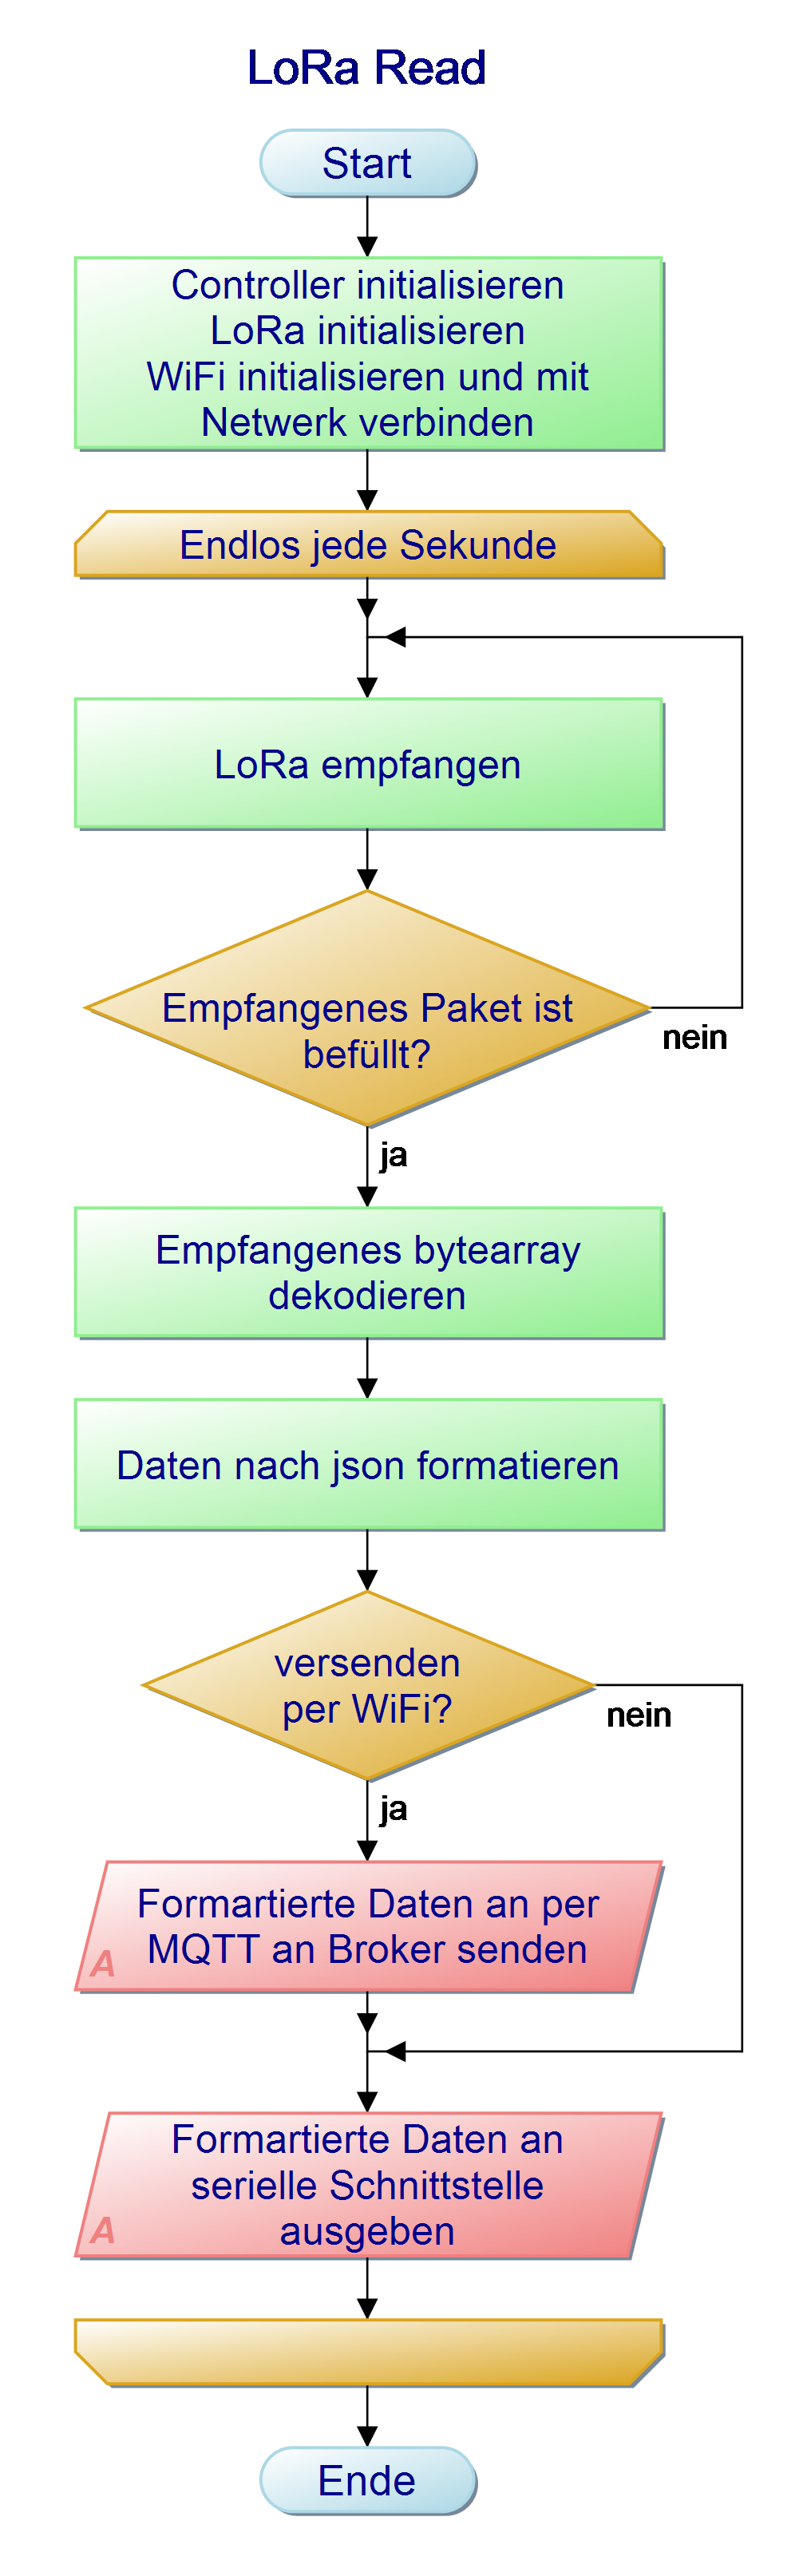
\includegraphics[width=0.3\textwidth]{pictures/LoRaRead}}
	 \caption[PAP komponente 2]{Programm Ablauf: Komponente 2}
	 \label{fig:lorareadwifisend}
	\end{figure}
\end{center}

Diese Softwarekomponente läuft schlussendlich auf dem LoRa Gateway, bzw. in unserem Fall dem zweiten Microcontroller, welcher in unserem Fall den Empfänger bei der P2P Verbindung darstellt.
Wie bei der ersten Komponente, wird zunächst der Microcontroller initialisiert. Des Weiteren werden Konfigurationsdaten eingelesen, welche für die optionale WiFi Verbindung und das senden an die MQTT Broker benötigt werden. Möchte man die Sensordaten einfach nur über eine serielle Schnittstelle auslesen, können diese Felder entsprechend leer gelassen werden.
Außerdem wird in dieser Komponente das LoRa Modul direkt initialisiert, da dies nur einmalig geschehen muss.\\
Es beginnt eine Endlosschleife, welche in bestimmten Abständen schaut, ob an dem Socket neue, per LoRa emfpangene, Daten aufgetaucht sind. Sollte dies der fall sein, werden die empfangenens bytes decodiert und auf ihre plausibilität gebprüft. Machen die empfangenen Daten Sinn, werden sie ins JSON Format gebracht und über die Serielle Schnitstelle ausgegeben, sollte der Nutzer der Microcontroller mit dem Internet verbunden haben, werden die Daten per MQTT an die entsprechenden Broker gesendet.\\
In der Konfigurationsdatei kann der Nutzer bestimmte Schwellwerte definieren, bei denen die Daten an unterschiedliche Broker gesendet werden. Somit können auf dem einen Feed zunächst alle Daten gesammelt werden, auf einem anderen wiederum, nur Daten die einen wirklich interessieren.

\subsection{3. Komponente: Manuelles abrufen und versenden der veröffentlichten Daten} \label{PubSub}

Möchte der Nutzer seine Daten zunächst nur lokal verwalten, hat er dennoch die Möglichkeit mithilfe der beiden folgende Skripte die Daten Nachträglich per MQTT an einen Broker zu schicken, bzw. den entsprechenden MQTT Broker zu subscriben, um seine Daten an einer anderen Stelle für die weitere Verabeitung zu sammeln.\\

\begin{center}
	\begin{figure}[h]
	 
	 \noindent\makebox[\textwidth]{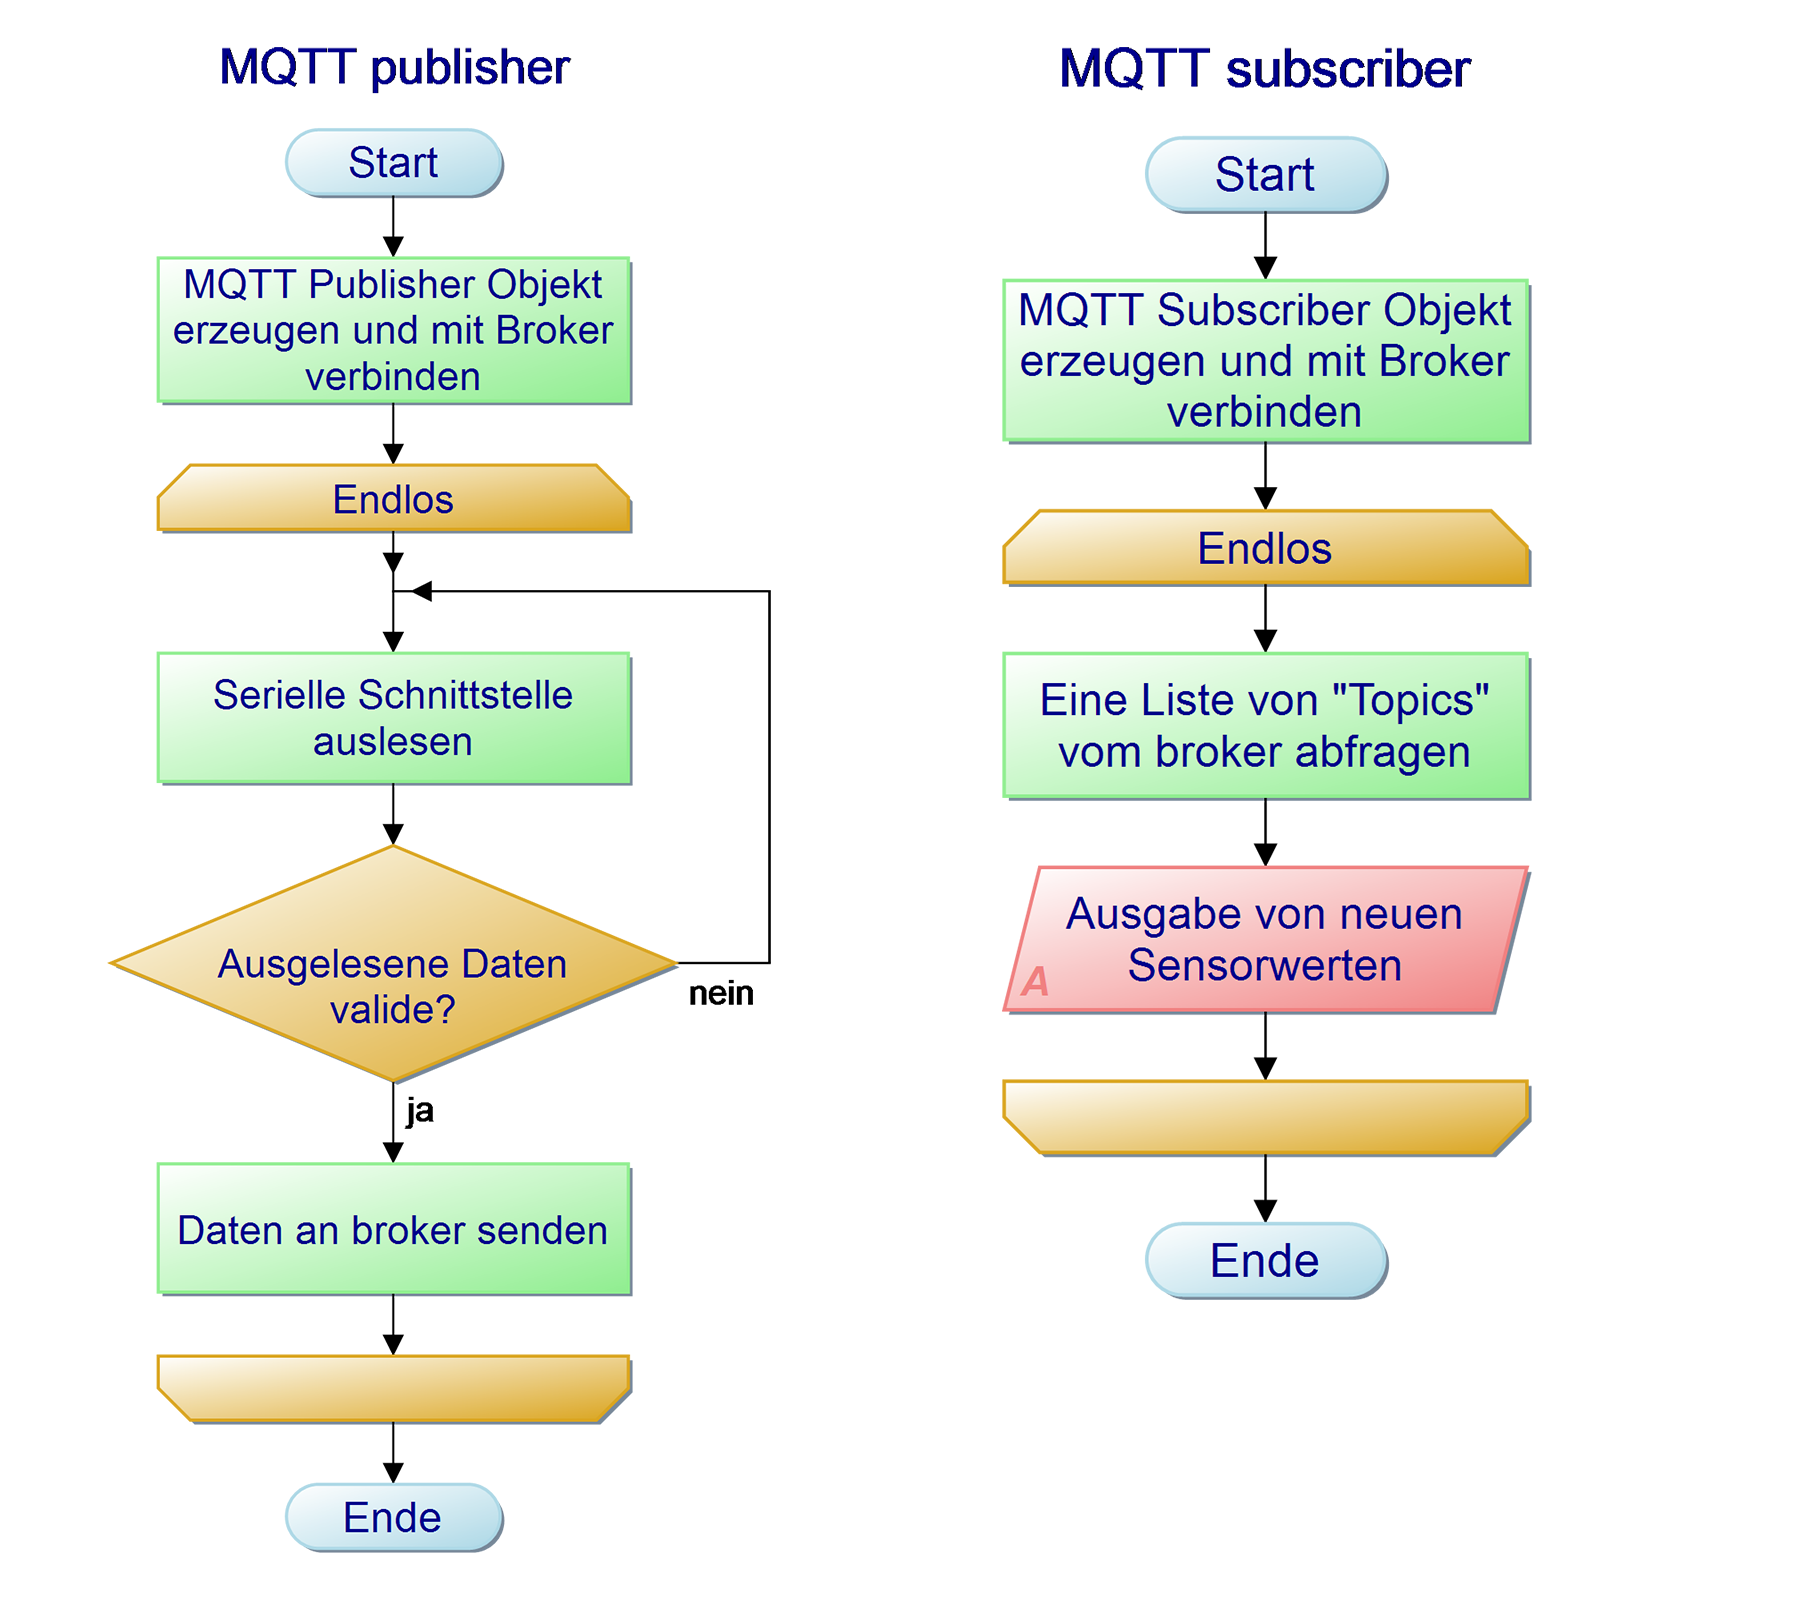
\includegraphics[width=0.9\textwidth]{pictures/MQTTpubsub}}
	 \caption[PAP komponente 3]{Programm Ablauf: Komponente 3}
	 \label{fig:MQTTpubsub}
	\end{figure}
\end{center}
=======
Es beginnt eine Endlosschleife

\newpage



\section{Visualisierung der Sensordaten} \label{Dashboard und Visualisierung}

\ldots


\section{Berechnung der Laufzeit im Batteriebetrieb} \label{Simulation}

\begin{center}
	\begin{figure}[h]
	 
	 \noindent\makebox[\textwidth]{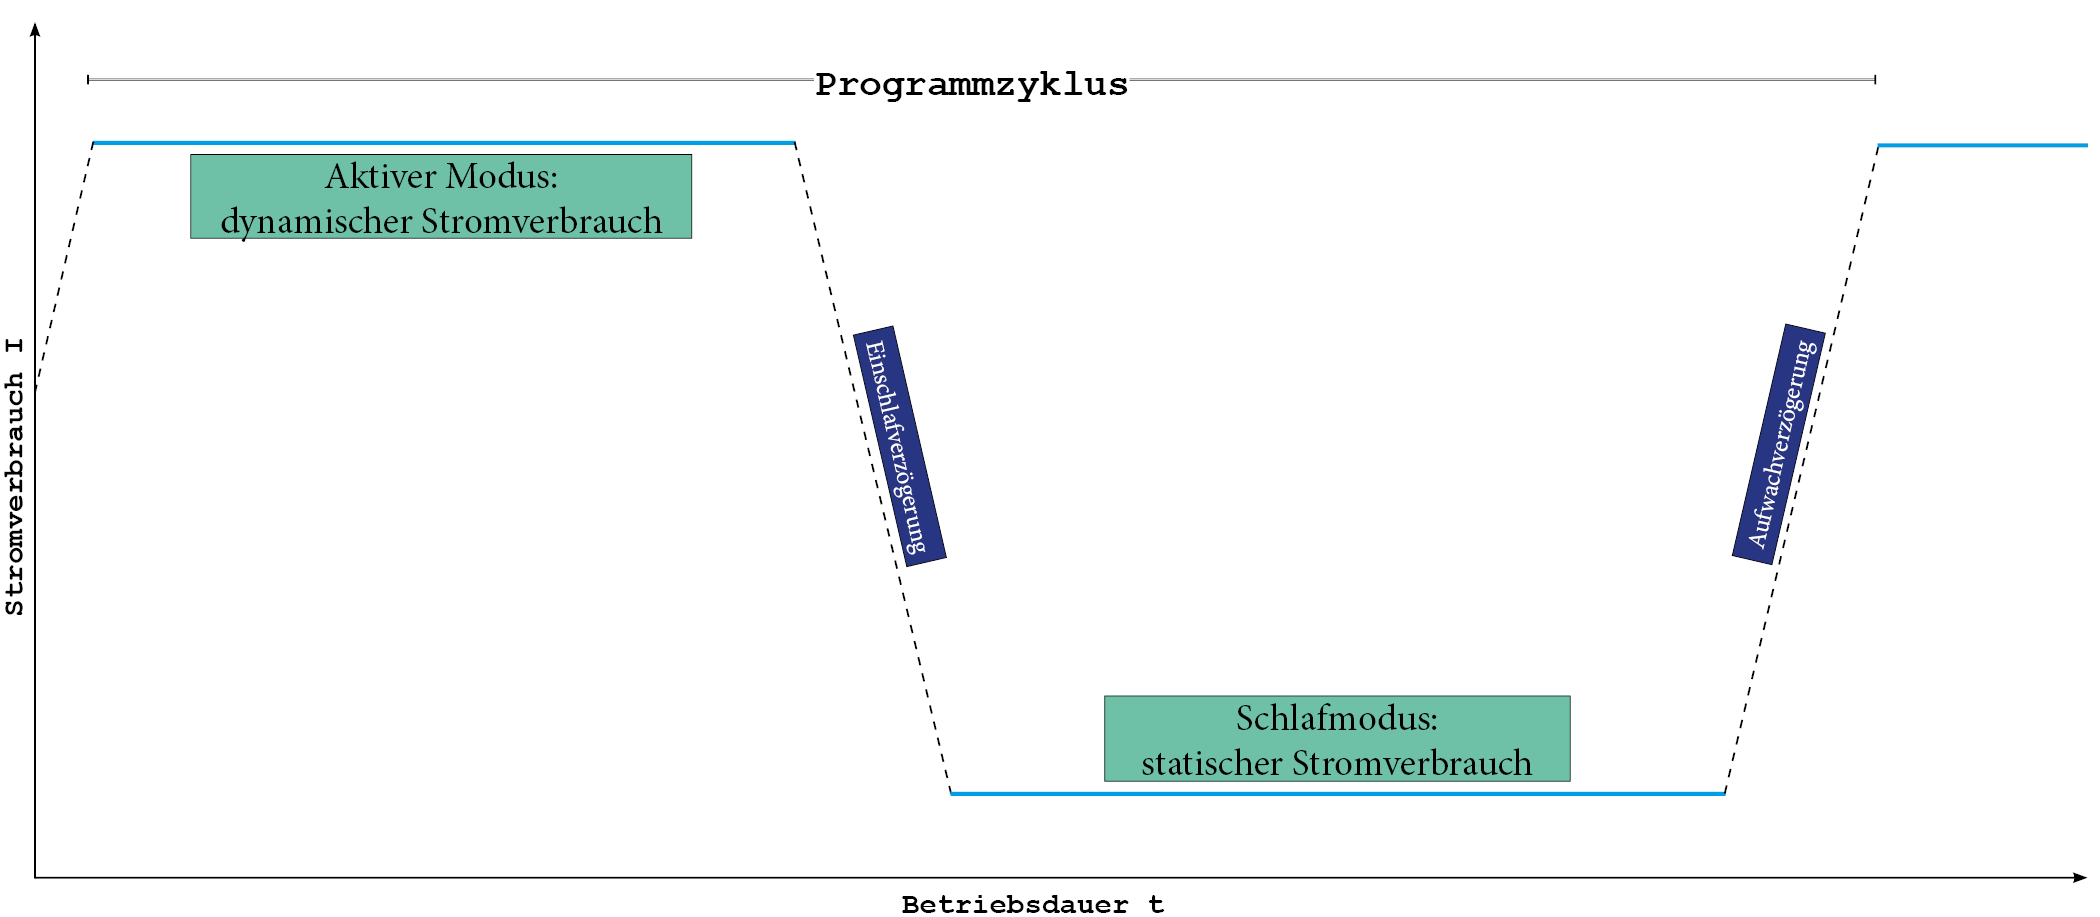
\includegraphics[width=1.1\textwidth]{pictures/programmzyklus}}
	 \caption[Stromverbrauch während eines Programmzyklus]{Stromverbrauch während eines Programmzyklus}
	 \label{fig:stromzyklus}
	\end{figure}
\end{center}

\[I_{avg} = \frac{I_{aktiv}\cdot t_{aktiv} + I_{passiv} \cdot t_{passiv}}{t_{aktiv} + t_{passiv}}\]

\[t_{Laufzeit} = \frac{C_{Batterie}}{I_{avg}}\]

\newpage



% !TEX root = ../Abschlussbericht_Schimmeliger_Keller.tex
%%
%%  Hochschule für Technik und Wirtschaft Berlin --  Projektabschlussbericht
%%
%% Kapitel 5 - Fazit
%%
%%

\chapter{Fazit} \label{Fazit}

\section{Projektauswertung} \label{Projektauswertung}

\subsubsection{Sidney}
Insgesammt war es für mich ein sehr interessantes Projekt gewesen. Für mich war es besonder interessant, zu erfahren, dass scheinbar doch eine Menge Initiativen und Projekte existieren, die ihren Fokus auf das Commoning bzw. auf das bereitstellen von freien Inhalten legen.\\
Für mich persönlich ging es in der Veranstaltung allerdings zu sehr um die Idee, ein Produkt zu vermarkten, wo wiederum jeder seinen eigenen Schwerpunkt legt.\\

\subsubsection{Ilja}
Durch die Durchführung des Projektes, angefangen mit der Auswahl der Projektteilnehmer und der Generierung der Projektideen in den einzelnen Workshops,
die von Hanna so toll und gruppendynamisch geleitet wurden, bis zur Durchführung der Umfragen bei Freunden und Bekannten, der Planung und schließlich der Umsetzung der Projektidee, habe ich persönlich viel mitgenommen und dazugelernt. \\
Außerdem hat es sehr viel Spaß gemacht, gemeinsam an etwas zu arbeiten, bei dem es im Vordergrund nicht um den Profit oder die maximale Gewinnerbringung geht, was im Grunde auch das Prinzip des Commoning ist, sondern, wie Sidney schon erwähnt hat, um eine gewisse Philosophie und eine Vision einen Mehrwert für die Community/Gesellschaft zu generieren. Es geht um aktive Mitbeteiligung, damit man nicht nur ein Konsument, sondern selbst auch ein Produzent sein kann und sich als Teil der Gesellschaft fühlt und anerkannt wird.

\section{Probleme und Herausforderungen} \label{Probleme und Herausforderungen}

\subsubsection{Sidney}
Neben kleineren Problemen wie z.B. einem falschen USB-Kabel, war es wie so häufig eher das Problem, den Fokus auf die wichtigen Dinge zu legen, wobei aber der Projektmanagement-Anteil definitiv geholfen hat, etwas struktur in den ganzen Djungel zu bringen.

\subsubsection{Ilja}
Die ersten Herausforderungen gab es zum einen bei der Beschaffung der notwendigen Hardware. So haben wir uns am Anfang viel damit auseinandergesetzt, wie man überhaupt Wasserschäden im Keller messen kann. Es gab die Überlegungen Sensoren zu verwenden, die die relative Feuchtigkeit im Beton messen würden, aber dafür müsste man ein Loch in den Boden bohren und das wäre natürlich nicht so schön. Außerdem fallen diese Art von Sensoren normalerweise recht teuer aus. Später haben wir uns auf klassischen Luftfeuchtigkeitssensor entschieden, der die relative Luftfeuchtigkeit misst. Das reicht eigentlich auch aus, da damit quasi schon der Wassergehalt in der Luft angegeben wird und wenn dieser Wert zu lange in einem hohen Bereich liegt, dann kann es passieren, dass sich der Beton wie ein Schwamm vollsaugt und sich dadurch Schimmel bildet und damit auch Wasserschäden entstehen.\\
Durch die Unterstützung von Prof. Scheffler, haben wir außerdem noch zwei Development-Boards mit LoRa-Modulen erhalten. Dies hat uns eine Menge Arbeit erspart, seperat einen LoRa-Chip und Mikrocontroller bestellen und diese noch konfigurieren zu müssen. \\
Jedoch hatte ich am Anfang, da ich Linux als Betriebssystem verwende, einige Schwierigkeiten mit der Installation des Pymakr-Plugins für den Upload bzw. das Flashen des Codes auf den Mikrocontroller. Somit musste ich ständig den Code via FTP auf das Board rüberkopieren, was sehr umständlich war, da man zuerst einen FTP-Server auf dem Mikrocontroller einrichten, der wiederum eine IP-Addresse von dem AP/Router bekommen musste... Aber Schlussendlich hat es dann doch geklappt und wir konnten, bis auf das LoRaWAN, unsere Projektidee realisieren.


\section{Ausblick} \label{Ausblick}

\subsubsection{Erweiterung von LoRa-LoRa zu LoRaWAN}
In unserem Projekt haben wir bisher leider kein richtiges Sensornetzwerk aufgebaut, sondern zwei Microcontroller über eine P2P LoRa Verbindung Kommunizieren lassen. Dies hat zum einen den Grund, dass wir selber kein LoRa Gateway aufbauen wollten, zum anderen aber auch kein umliegendes Gateway in erreichbarer Nähe haben.

\subsubsection{Benutzung von mehreren Sensorknoten an einem LoRa-Gateway}
Wenn wir es hinbekommen sollten ein eigenes Gateway bereitzustellen, welches auch unsere Publisher-Software implementiert hat, würden wir gerne mehrere Sensorknoten mit diesem Gateway verbinden, um so möglicherweise Unterschiede in den Messdaten zwischen den Microcontrollern zu entdecken.

\subsubsection{Erweiterung der Software zur Einbindung von mehreren Sensorkomponenten}
Derzeit haben bieten wir nur die Möglichkeit einen oder mehrere DHT Sensoren einzubinden. Wir würden gerne eine universelle Schnittstelle bereitstellen, die es ermöglicht eine Vielzahl von Sensoren anzubinden und auszuwerten.

\subsubsection{Batteriebetrieb in Hardware umsetzen}
Den Batteriebetrieb haben wir bisher nur Simuliert. Da wir keine geeigneten Konstruktion bauen konnten, die einen Batteriehalter ordnungsgemäß halten könnte. Zu einem Serienreifen Produkt gehört somit auch ein Gehäuse mit Battriehalter.

\subsubsection{Alternative Dashboard Möglichkeiten}
Wir würden gerne weitere Dashboardmöglichkeiten evalueiren, da die kostenlose Version der \textit{adafruit.io} Dashboards doch recht limiert ist. Ggf. ist es auch Sinnvoll eine eigene Dashboard Plattfrom bereitzustellen, da wir weiterhin den Ansatz der freien Inhalte verfolgen wollen.

\section{Abschlusswort} \label{Abschlusswort}

Peace



%% Anhang
\cleardoubleoddpage
\appendix
% !TEX root = ../Thesis.tex
%%
%%  Hochschule für Technik und Wirtschaft Berlin --  Projektabschlussbericht
%%
%% Anhang
%%
%%%%%%%%%%%%%%%%%%%%%%%%%%%%%%%%%%%%%%%%%%%%%%%%%%%%%%%%%%%%%%%%%%%%%


\chapter{Anhang}


\ldots

%%%%%%%%%%%%%%%%%%%%%%%%%%%%%%%%%%%%%%%%%%%%%
%%%%%%%%%%%%%%%%%%%%%%%%%%%%%%%%%%%%%%%%%%%%%
%%%%%%%%%%%%%%%%%%%%%%%%%%%%%%%%%%%%%%%%%%%%%


%% Abkürzungsverzeichnis
% 	Befehl: makeindex Thesis.nlo -s nomencl.ist -o Thesis.nls
%
% !TEX root = ../Thesis.tex
%%
%%  Hochschule für Technik und Wirtschaft Berlin --  Abschlussarbeit
%%
%%  Abkürzungsverzeichnis
%%
%% Vorgeplänkel nach
%% http://blog.stefan-macke.com/2006/05/03/abkurzungsverzeichnis-mit-latex/
%%%%%%%%%%%%%%%%%%%%%%%%%%%%%%%%%%%%%%%%%%


\acro{EU}{Europäische Union}
\acro{6LoWPAN}{IPv6 over Low power Wireless Personal Area Network}
\acro{AC}{Alternating Current (Wechselstrom)}
\acro{ANSI}{American National Standards Institute}
\acro{PDU}{Protocol Data Unit}
\acro{API}{Application Programming Interface}
\acro{APS}{Application Support Sublayer (ZigBee)}
\acro{ASDU}{Application Service Data Unit}
\acro{BAN}{Body Area Network}
\acro{BSD}{Berkeley Software Distribution}


\cleardoublepage
\markboth{\nomname}{\nomname}
\printnomenclature

%% Abbildungsverzeichnis
\listoffigures \clearpage

%% Tabellenverzeichnis
\listoftables \clearpage

%% Quelltextverzeichnis
\lstlistoflistings \clearpage

%% Stichwortverzeichnis
%	Befehl: makeindex Thesis
%
\printindex \clearpage

%% Literaturverzeichnis
%   Befehl: biber Thesis
%
\printbibliography[heading=bibintoc, title={\babel{Literaturverzeichnis}{Bibliography}}]
\clearpage
%Literaturverzeichnisse getrennt nach Stichwort
%\printbibliography[heading=bibintoc, keyword={book}, title={Literaturverzeichnis}]\clearpage
%\printbibliography[heading=bibintoc, keyword={online}, title={Onlinequellen}]\clearpage
%\printbibliography[heading=bibintoc, keyword={image}, title={Bildquellen}]\clearpage

%% Erklärung zur Eigenständigkeit
% !TEX root = Thesis.tex
%%
%%  Hochschule für Technik und Wirtschaft Berlin --  Abschlussarbeit
%%
%%  Erklärung zur Eigenständigkeit
%%
%%%%%%%%%%%%%%%%%%%%%%%%%%%%%%%%%%%%%%%%%%%%%%%%%%%%

\addchap{Eigenständigkeitserklärung}

Hiermit versichern wir, dass wir das vorliegende \thethesistyp{} selbstständig und nur unter
Verwendung der angegebenen Quellen und Hilfsmittel verfasst haben. 

\vskip 1cm

Berlin, den \thedatum

\vskip 1.5cm

\theautor


\end{document}
